\documentclass[fleqn, a4paper, 12pt, twoside]{article}
\usepackage{exsheets} %question and solution environments
\usepackage{amsmath, amssymb, amsthm} %standard AMS packages
\usepackage{esint} %integral signs
\usepackage{marginnote} %marginnotes
\usepackage{gensymb} %miscellaneous symbols
\usepackage{commath} %differential symbols
\usepackage{xcolor} %colours
\usepackage{cancel} %cancelling terms
\usepackage{siunitx} %formatting units
\usepackage{tikz, pgfplots} %diagrams
	\usetikzlibrary{calc, hobby, patterns, intersections, angles, quotes, spy}
\usepackage{graphicx} %inserting graphics
\usepackage{epstopdf} %converting and inserting eps graphics
\usepackage{hyperref} %hyperlinks
\usepackage{datetime} %date and time
\usepackage{ulem} %underline for \emph{}
\usepackage{xfrac, lmodern} %inline fractions
\usepackage{enumerate, enumitem} %numbered lists
\usepackage{float} %inserting floats
\usepackage[american voltages]{circuitikz} %circuit diagrams
\usepackage{pdflscape}
\usepackage{setspace}
\usepackage{microtype}

\newcommand\numberthis{\addtocounter{equation}{1}\tag{\theequation}} %adds numbers to specific equations in non-numbered list of equations

\newcommand{\AxisRotator}[1][rotate=0]{
	\tikz [x=0.25cm,y=0.60cm,line width=.2ex,-stealth,#1] \draw (0,0) arc (-150:150:1 and 1);%
} %rotation symbols on axes

\theoremstyle{definition}
\newtheorem{example}{Example}
\newtheorem{definition}{Definition}

\theoremstyle{theorem}
\newtheorem{theorem}{Theorem}
\newtheorem{law}{Law}

\newcommand{\curl}{\mathrm{curl\,}}

\newcommand{\divergence}{\mathrm{div\,}}

\makeatletter
\@addtoreset{section}{part} %resets section numbers in new part
\makeatother

\newcommand\blfootnote[1]{%
	\begingroup
	\renewcommand\thefootnote{}\footnote{#1}%
	\addtocounter{footnote}{-1}%
	\endgroup
}

\SetupExSheets{solution/print = true} %prints all solutions by default

%opening
\title{Physics 2}
\author{Aakash Jog}
\date{2014-15}

\begin{document}

\maketitle
%\setlength{\mathindent}{0pt}

\blfootnote
{	
	\begin{figure}[H]
		\includegraphics[height = 12pt]{cc.eps}
		\includegraphics[height = 12pt]{by.eps}
		\includegraphics[height = 12pt]{nc.eps}
		\includegraphics[height = 12pt]{sa.eps}
	\end{figure}
	This work is licensed under the Creative Commons Attribution-NonCommercial-ShareAlike 4.0 International License. To view a copy of this license, visit \url{http://creativecommons.org/licenses/by-nc-sa/4.0/}.
} %CC-BY-NC-SA license

\tableofcontents

\newpage
\section{Lecturer Information}

\textbf{Dr. Erez Pyetan}\\
~\\
Office: Sharet 325\\
Telephone: 7565\\
E-mail: erezpyet@mail.tau.ac.il\\

\section{Textbooks}

\begin{enumerate}
	\item D. Halliday, R. Resnick, and K. S. Krane: \textit{Physics}, 5th edition, vol. 2 (Wiley)
	\item D.J. Griffiths: \textit{Introduction to Electrodynamics}
\end{enumerate}

\newpage
\part{Electrostatics}

\section{Coulomb's Law}

\begin{law}[Coulomb's Law]
	The force between two charged particles is directly proportional to the product of the charges of the particles, and inversely proportional to the square of the distance between them.
	\begin{align*}
		F &\propto \dfrac{q_1 q_2}{r^2}\\
		F &= k \dfrac{q_1 q_2}{r^2}\\
		&= \dfrac{1}{4 \pi \varepsilon_0} \cdot \dfrac{q_1 q_2}{r^2}
	\end{align*}
	The constant of proportionality is $k = 8.99 \times 10^9 \si{\newton\metre\squared\per\coulomb\squared}$.\\
	$\varepsilon_0 = 8.8541878162 \times 10^{-12} \si{\coulomb\squared\per\newton\per\metre\squared}$ is called the permittivity of free space.\\
	In vector notation,
	\begin{align*}
		\overrightarrow{F_{2 1}} &= \dfrac{1}{4 \pi \varepsilon_0} \dfrac{q_1 q_2}{{r_{1 2}}^2} \hat{r_{1 2}}
	\end{align*}
	\label{Coulomb's_Law}
\end{law}
~\\
Charge is defined according to this law.\\

\begin{question}
	A charge $q$ is placed at the origin. A charge $-2q$ is placed at 1 \si{\metre} from it, in the $x$ direction. Find a point on the $y$-axis where the total force acting on a charge $q'$ will be parallel to the $x$-axis.\\
\end{question}

\begin{solution}
	\begin{figure}[H]
		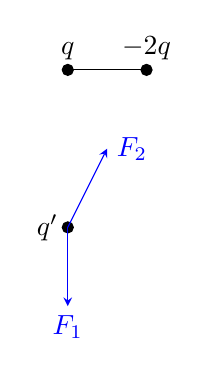
\begin{tikzpicture}
			\def\y{-2};
			\def\F{1};
			
			\coordinate (q) at (0,0);
			\coordinate (-2q) at (1,0);
			\coordinate (q') at (0,\y);
			
			\filldraw (q) circle [radius = 2pt] node [above] {$q$};
			\filldraw (-2q) circle [radius = 2pt] node [above] {$-2q$};
			\filldraw (q') circle [radius = 2pt] node [left] {$q'$};
			
			\draw (q) -- (-2q);
			
			\begin{scope}[blue, -stealth]
				\draw (q') -- ++(-90:\F) node [below] {$F_1$};
				\draw (q') -- ($ (q') ! 0.5 ! (-2q) $) node [right] {$F_2$};
			\end{scope}
		\end{tikzpicture}
	\end{figure}
	For the net force to be in the $x$ direction, the components of $F_1$ and $F_2$ in the $y$ direction must cancel each other out.
	\begin{align*}
		F_1 &= F_2 \sin \theta\\
		\therefore \cancel{k} \cdot \dfrac{(\cancel{q'})(-2\cancel{q})}{y^2 + 1} \cdot \dfrac{y}{\sqrt{y^2 + 1}} &= \cancel{k} \cdot \dfrac{(\cancel{q})(\cancel{q'})}{y^2}\\
		\therefore \dfrac{-2y}{(y^2 + 1)^{\sfrac{3}{2}}} &= \dfrac{1}{y^2}\\
		\therefore y &= \pm \sqrt{\dfrac{1}{2^{\sfrac{2}{3}}- 1}}
	\end{align*}
\end{solution}

\begin{question}
	A rod of length $L$ has a uniformly distributed charge $Q$, with line charge density $\lambda = \dfrac{Q}{L}$. A point charge $q$ is kept at a distance $x$ as shown.
	\begin{figure}[H]
		\begin{tikzpicture}
			\def\L{5};
			\def\x{10};
			
			\coordinate (q) at (\x,0);
			
			\draw [ultra thick] (0,\L/2) -- (0,-\L/2);
			
			\filldraw (q) circle [radius = 2pt] node [right] {$q$};
			
			\begin{scope}[|<->|]
				\draw [xshift = -20] (0,\L/2) -- (0,-\L/2) node [midway, fill = white] {$L$};
				\draw [xshift = -10] (0,\L/2) -- (0,0) node [midway, fill = white] {$\dfrac{L}{2}$};
			\end{scope}
		\end{tikzpicture}
	\end{figure}
\end{question}

\begin{solution}
	\begin{figure}[H]
		\begin{tikzpicture}
			\def\L{5};
			\def\x{10};
			\def\y{0.75*\L/2};
			\def\dy{0.1*\y};
			
			\coordinate (q) at (\x,0);
			\coordinate (dq) at (0, {\y + (\dy/2)});
			
			\draw [ultra thick] (0,\L/2) -- (0,-\L/2);
			
			\filldraw (q) circle [radius = 2pt] node [above] {$q$};
			
			\begin{scope}[dashed]
				\draw (q) -- (dq) node [midway, fill = white] {$r = \sqrt{x^2 + y^2}$};
				\draw (q) -- (0,0);
			\end{scope}
			
			\begin{scope}[red, -stealth]
				\draw (q) -- ($(q) ! -1cm ! (dq)$) node [below right] {$\dif F$};
			\end{scope}
			
			\draw [|<->|, yshift = -10] (0,0) -- (\x,0) node [midway, fill = white] {$x$};
			\draw [|<->|, xshift = -10] (0,0) -- (0,\y) node [midway, fill = white] {$y$};
			
			\draw [|-|, xshift = -10] (0,\y) -- ++(0,\dy) node [midway, left] {$\dif y$};
		\end{tikzpicture}
	\end{figure}
	The $y$ components of the forces of the elemental charges at $y$ and $-y$ on $q$ are cancelled out. Therefore, the net force is in the $x$ direction only.
	\begin{align*}
		\dif F &= k \dfrac{(\dif Q) (q)}{r^2}\\
		\dif F_x &= \dif F \cos \theta\\
		&= k \dfrac{(\dif Q) (q)}{r^2} \cos \theta\\
		&= k \dfrac{(\lambda \dif y) (q)}{x^2 + y^2} \dfrac{x}{\sqrt{x^2 + y^2}}\\
		&= k \lambda q x \dfrac{\dif y}{(x^2 + y^2)^{\sfrac{3}{2}}}\\
		\therefore \overrightarrow{F} &= \hat{x} \int \dif F_x\\
		&= \hat{k} \lambda q x \int\limits_{-\sfrac{L}{2}}^{\sfrac{L}{2}} \dfrac{\dif y}{(x^2 + y^2)^{\sfrac{3}{2}}}
	\end{align*}
		Substituting $y = x \tan \theta$ and $\dif y = x \sec^2 \theta \dif \theta$
	\begin{align*}
		\overrightarrow{F} &= \hat{x} \lambda q k x \int\limits_{-\theta_0}^{\theta_0} \dfrac{1}{x^2} \cos \theta \dif \theta\\
		&= \hat{x} \dfrac{\lambda q k}{x} \int\limits_{-\theta_0}^{\theta_0} \cos \theta \dif \theta
	\end{align*}
		Therefore,
	\begin{align*}
		\overrightarrow{F} &= \hat{x} \dfrac{2 \lambda q k}{x} \sin \theta_0\\
		&= \hat{x} \dfrac{2 \lambda q k}{x} \dfrac{\dfrac{L}{2}}{\left( \left( \dfrac{L}{2} \right)^2 + x^2 \right)^{\sfrac{1}{2}}}\\
		&= \hat{x} \dfrac{2 \left( \dfrac{Q}{L} \right) q k}{x} \cdot  \dfrac{\dfrac{L}{2}}{\left( \left( \dfrac{L}{2} \right)^2 + x^2 \right)^{\sfrac{1}{2}}}\\
		&= k \dfrac{Q q}{x \left( \left( \dfrac{L}{2} \right)^2 + x^2 \right)^{\sfrac{1}{2}}} \hat{x}
	\end{align*}
\end{solution}

\begin{question}
	A point charge $q$ is kept at a distance $z$ above a ring of radius $R$ charged with $Q = 2 \pi R \lambda$, where $\lambda$ is the linear charge density. Find the force acting on $q$.
\end{question}

\begin{solution}
	\begin{figure}[H]
		\begin{tikzpicture}
			\def\R{3};
			\def\z{5};
			
			\coordinate (q) at (0,\z);
			\coordinate (dQ) at (-\R,0);
			
			\draw (0,0) circle [x radius = \R, y radius = 0.4*\R];
			
			\filldraw (q) circle [radius = 2pt] node [above] {$q$};
			
			\begin{scope}[dashed]
				\draw (0,0) -- (q);
				\draw (0,0) -- (dQ);
				\draw (q) -- (dQ) node [midway, fill = white] {$\sqrt{z^2 + R^2}$};
			\end{scope}
		\end{tikzpicture}
	\end{figure}
	Due to the symmetry of the ring, the net force acting on $q$ is in the $z$ direction only.
	\begin{align*}
		\dif F_z &= \dif F \cos \theta\\
		&= k \dfrac{(\dif Q) (q)}{z^2 + R^2} \cos \theta\\
		&= k \dfrac{(\dif Q) (q)}{z^2 + R^2} \dfrac{z}{\sqrt{z^2 + R^2}}\\
		&= k q z \dfrac{\dif Q}{\left( z^2 + R^2 \right)^{\sfrac{3}{2}}}\\
		\therefore \overrightarrow{F} &= \hat{z} \int \dif F_z\\
		&= \hat{z} k q z \dfrac{1}{\left( z^2 + R^2 \right)^{\sfrac{3}{2}}} \int\limits_{0}^{Q} \dif Q\\
		&= k \dfrac{Q q z}{\left( z^2 + R^2 \right)^{\sfrac{3}{2}}} \overrightarrow{z}
	\end{align*}
\end{solution}

\begin{question}
	A point charge $q$ is kept at a distance $z$ above a disk of radius $R$ charged with $Q = \pi R^2 \sigma$, where $\sigma$ is the surface charge density. Find the force acting on $q$.
\end{question}

\begin{solution}
	The disk can be considered to be made up of elemental rings, with radii varying from $0$ to $R$.\\
	Therefore,
	\begin{align*}
		\dif \overrightarrow{F} &= k \dfrac{q Q_{\textnormal{ring}}}{\left( z^2 + R^2 \right)^{\sfrac{3}{2}}} \hat{z}\\
		&= k \dfrac{q (\sigma \cdot 2 \pi r \cdot \dif r)}{\left( z^2 + R^2 \right)^{\sfrac{3}{2}}} z \hat{z}
	\end{align*}
	Hence,
	\begin{align*}
		\overrightarrow{F} &= \int \dif\overrightarrow{F}\\
		&= \hat{z} \int\limits_{0}^{R} k \dfrac{q \sigma \cdot 2 \pi r z \cdot \dif r}{\left( z^2 + R^2 \right)^{\sfrac{3}{2}}}\\
		&= 2 k z q \sigma \pi \left( \dfrac{1}{|z|} - \dfrac{1}{\sqrt{z^2 + R^2}} \right)\hat{z}
	\end{align*}
	If $z << R$, i.e. for an infinite sheet,
	\begin{align*}
		F &= 2 q \sigma \pi k 
	\end{align*}
\end{solution}

\section{Electric Field}

\begin{definition}[Electric field]
	The electric field at a point in space is the electric force felt by a charge of 1 \si{\coulomb} had it been kept there.
\end{definition}

\subsection{Standard Electric Fields}

\begin{tabular}{l l}
	Line of charge & $\dfrac{1}{4 \pi \varepsilon_0} \dfrac{\lambda L}{r \sqrt{r^2 + \dfrac{L^2}{4}}}$\\
	Infinite line of charge & $\dfrac{\lambda}{2 \pi \varepsilon_0 r}$\\
	Ring of charge & $\dfrac{\lambda R z}{2 \varepsilon_0 \left( z^2 + R^2 \right)^{\sfrac{3}{2}}}$\\
	Infinite plane of charge & $\dfrac{\sigma}{2 \varepsilon_0}$
\end{tabular}

\subsection{Capacitors}

A parallel plate capacitor is constructed by arranging two infinite plates with surface charge density $\sigma$ and $-\sigma$ respectively.
\begin{figure}[H]
	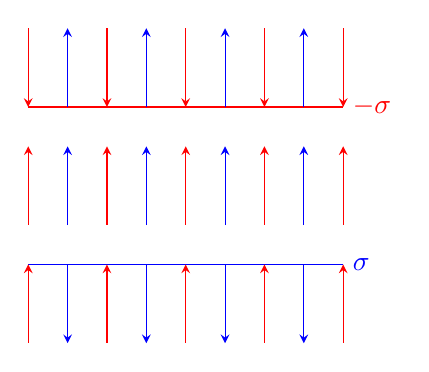
\begin{tikzpicture}
		\def\l{4};
		\def\d{2};
		
		\draw [blue] ({-\l/2}, {-\d/2}) -- ({\l/2}, {-\d/2}) node [right] {$\sigma$};
		\draw [red] ({-\l/2}, {\d/2}) -- ({\l/2}, {\d/2}) node [right] {$-\sigma$};
		
		\begin{scope}[blue, -stealth]
			\foreach \i in {-1.5,...,1.5}
				\draw (\i,{-\d/4}) -- ++(0,1);
		\end{scope}
		
		\begin{scope}[blue, -stealth]
			\foreach \i in {-1.5,...,1.5}
				\draw (\i,{\d/2}) -- ++(0,1);
		\end{scope}
		
		\begin{scope}[blue, -stealth]
			\foreach \i in {-1.5,...,1.5}
				\draw (\i,{-\d/2}) -- ++(0,-1);
		\end{scope}
		
		\begin{scope}[red, stealth-]
			\foreach \i in {-2,...,2}
				\draw (\i,{\d/4}) -- ++(0,-1);
		\end{scope}
		
		\begin{scope}[red, stealth-]
			\foreach \i in {-2,...,2}
				\draw (\i,{\d/2}) -- ++(0,1);
		\end{scope}
		
		\begin{scope}[red, stealth-]
			\foreach \i in {-2,...,2}
				\draw (\i,{-\d/2}) -- ++(0,-1);
		\end{scope}
	\end{tikzpicture}
\end{figure}

The electric field due to the plates are as shown. 
Therefore, the fields between the plates add up and the fields outside the plates cancel out.\\
Therefore, the net field inside the capacitor is 
\begin{equation*}
	{\color{red} \dfrac{\sigma}{2 \varepsilon_0}} + {\color{blue} \dfrac{\sigma}{2 \varepsilon_0}} = \dfrac{\sigma}{\varepsilon_0}
\end{equation*}

\section{Electric Dipoles}

\begin{definition}[Electric dipole]
	Two charges, $q$ and $-q$, separated by a distance $d$ is called an electric dipole.
	\begin{figure}[H]
		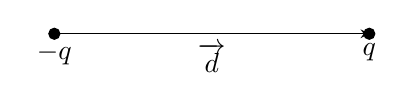
\begin{tikzpicture}
			\def\d{4};
			
			\draw [-stealth] ({-\d/2},0) -- ({\d/2},0) node [midway, below] {$\overrightarrow{d}$};
			
			\filldraw ({-\d/2},0) circle (2pt) node [below] {$-q$};
			\filldraw ({\d/2},0) circle (2pt) node [below] {$q$};
		\end{tikzpicture}
	\end{figure}
\end{definition}

\begin{definition}[Dipole moment]
	If two charges $q$ and $-q$ are separated by a distance $d$, the dipole moment is defined as
	\begin{equation*}
		\overrightarrow{P} \doteq q \cdot \overrightarrow{d}
	\end{equation*}
	where $\overrightarrow{d}$ is the vector of length $d$ pointing from $-q$ to $q$.
\end{definition}

\subsection{Electric Field Due to Electric Dipoles}

\subsubsection{Electric Field}

\begin{figure}[H]
	\begin{tikzpicture}
		\def\d{4};
		\def\x{3};
		
		\coordinate (O) at (0,0);
		\coordinate (+q) at (0,{\d/2});
		\coordinate (-q) at (0,{-\d/2});
		\coordinate (x) at (\x,0);
		
		\begin{scope}[-stealth, lightgray]
			\draw ({-(\x + 1)},0) -- ({\x + 1},0) node [right] {$x$};
			\draw (0,{-(\d/2 + 1)}) -- (0,{\d/2 + 1}) node [above] {$z$};
		\end{scope}
		
		\filldraw (+q) circle (1pt);
		\filldraw (-q) circle (1pt);
		
		\begin{scope}[xshift = -10, |<->|]
			\draw (0,0) -- (0,{\d/2}) node [midway, fill = white] {$\dfrac{d}{2}$};
			\draw (0,0) -- (0,{-\d/2}) node [midway, fill = white] {$\dfrac{d}{2}$};
		\end{scope}
		
		\begin{scope}[dashed, blue]
			\draw (\x,0) -- (+q) node [midway, above right] {$\sqrt{\dfrac{d^2}{4} + z^2}$};
			\draw (\x,0) -- (-q) node [midway, below right] {$\sqrt{\dfrac{d^2}{4} + z^2}$};
		\end{scope}
		
		\begin{scope}[-stealth, blue]
			\draw (\x,0) -- ($ (\x,0) ! -1cm ! (+q) $);
			\draw (\x,0) -- ($ (\x,0) ! 1cm ! (-q) $);
		\end{scope}
		
		\pic [draw,  "$\theta$", angle eccentricity = 1.5] {angle = O--+q--x};
	\end{tikzpicture}
\end{figure}

\begin{align*}
	\overrightarrow{F} &= 2 E_+ \cos \theta (- \hat{z})\\
	&= 2 \cdot \dfrac{1}{4 \pi \varepsilon_0} \dfrac{q}{\left( \dfrac{d}{2} \right)^2 + x^2} \cdot \dfrac{\dfrac{d}{2}}{\left( \left( \dfrac{d}{2} \right)^2 + x^2 \right)^{\sfrac{1}{2}}} (- \hat{z})\\
	&= - \dfrac{1}{4 \pi \varepsilon_0} \dfrac{\overrightarrow{P}}{\left( \left( \dfrac{d}{2} \right)^2 + x^2 \right)^{\sfrac{3}{2}}}
\end{align*}

\section{Gauss' Law}

\begin{definition}[Electric flux]
	Electric flux is defined as the dot product of the electric field passing through a surface, and the area vector of the surface.
	\begin{equation*}
		\Phi = \overrightarrow{E} \cdot \overrightarrow{A}
	\end{equation*}
	where the magnitude of the area vector is proportional to the area of the surface and the direction is perpendicular to the surface.
\end{definition}

This can be modelled as water passing through a surface.

\begin{figure}[H]
	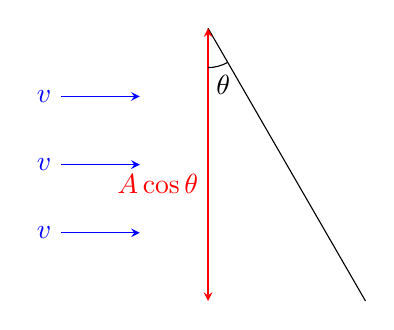
\begin{tikzpicture}
		\def\angle{30};
		\def\l{4};
		
		\coordinate (O) at (0,0);
		\coordinate (plate top) at (0,{\l*cos(\angle)});
		\coordinate (plate bottom) at ($ (plate top) + ({-90 + \angle}:\l) $);
		
		\draw (plate top) -- (plate bottom);
		
		\draw [red, stealth-stealth] (plate top) -- (O) node [midway, below left] {$A \cos \theta$};
		
		\begin{scope}[blue, stealth-]
			\draw ({-\l*cos(\angle)/4},{\l*cos(\angle)/4}) -- ++(180:1) node [left] {$v$};
			\draw ({-\l*cos(\angle)/4},{2*\l*cos(\angle)/4}) -- ++(180:1) node [left] {$v$};
			\draw ({-\l*cos(\angle)/4},{3*\l*cos(\angle)/4}) -- ++(180:1) node [left] {$v$};
		\end{scope}
		
		\pic [draw, "$\theta$", angle eccentricity = 1.5] {angle = O--plate top--plate bottom};
	\end{tikzpicture}
\end{figure}

The flux of the water passing through the area $A$ is $A v \cos \theta$.

\begin{law}[Gauss' Law]
	\begin{equation*}
		\oiint \overrightarrow{E} \cdot \overrightarrow{\dif A} = \dfrac{Q_{\textnormal{inside}}}{\varepsilon_0}
	\end{equation*}
	\label{Gauss'_Law}
\end{law}

\begin{question}
	A hollow sphere of radius $R$ has surface charge density $\sigma$. Find the field at a point at distance $r$ from the centre of the sphere.
\end{question}

\begin{solution}
	Consider the imaginary Gaussian surface as a sphere with radius $r$.
	\begin{figure}[H]
		\begin{tikzpicture}
			\def\R{3};
			\def\r{5};
			
			\begin{scope}
				\draw (0,0) circle (\R);
				\draw [dashed] (0,0) -- ++({360*rnd}:\R) node [midway, fill = white] {$R$};
			\end{scope}
			
			\begin{scope}[blue, dashed]
				\draw (0,0) circle (\r);
				\draw [dashed] (0,0) -- ++({360*rnd}:\r) node [midway, fill = white] {$r$};
			\end{scope}
			
		\end{tikzpicture}
	\end{figure}
	Using Gauss' Law over the Gaussian surface,
	\begin{align*}
		\oiint \overrightarrow{E} \cdot \overrightarrow{\dif A} &= \dfrac{Q_{\textnormal{total}}}{\varepsilon_0}\\
		\therefore \oiint E \dif A &= \dfrac{Q_{\textnormal{total}}}{\varepsilon_0}\\
		\therefore E \oiint \dif A &= \dfrac{Q_{\textnormal{total}}}{\varepsilon_0}\\
		\therefore E \cdot 4 \pi r^2 &= \dfrac{Q_{\textnormal{total}}}{\varepsilon_0}\\
		\therefore \overrightarrow{E} &= \dfrac{1}{4 \pi \varepsilon_0} \dfrac{Q_{\textnormal{total}}}{r^2} \hat{r}
	\end{align*}
\end{solution}
~\\
Similarly for $r < R$, $E = 0$.

\section{Electric Potential}

\begin{definition}[Electrical Potential]
	The electric potential due to a point charge $q$ is
	\begin{align*}
		\varphi \left( \overrightarrow{r} \right) &= \dfrac{1}{4 \pi \varepsilon_0} \dfrac{q}{r} + c
	\end{align*}
\end{definition}

If a charge $q$ in moved from point $\textnormal{A}$ to $\textnormal{B}$,
\begin{align*}
	W_{\textnormal{\textnormal{A}} \to \textnormal{B}} &= \int\limits_{\overrightarrow{r_{\textnormal{A}}}}^{\overrightarrow{r_{\textnormal{B}}}} \overrightarrow{E} \cdot \dif \overrightarrow{r}\\
	&= \int\limits_{r_{\textnormal{A}}}^{r_{\textnormal{B}}} \dfrac{1}{4 \pi \varepsilon_0} \dfrac{q}{r^2} \dif r\\
	&= \left. - \dfrac{1}{4 \pi \varepsilon_0} \dfrac{q}{r} \right|_{r_{\textnormal{A}}}^{r_{\textnormal{B}}}\\
	&= \dfrac{1}{4 \pi \varepsilon_0} \dfrac{q}{r_{\textnormal{A}}} - \dfrac{1}{4 \pi \varepsilon_0} \dfrac{q}{r_{\textnormal{B}}}
\end{align*}

Therefore,
\begin{align*}
	W_{\textnormal{A} \to \textnormal{B}} &= \varphi \left( \overrightarrow{r_A} \right) - \varphi \left( \overrightarrow{r_B} \right)\\
	\therefore \varphi \left( \overrightarrow{r_B} - \overrightarrow{r_A} \right) &= - \int\limits_{\overrightarrow{r_A}}^{\overrightarrow{r_B}} \overrightarrow{E} \cdot \dif \overrightarrow{r}
\end{align*}

\begin{question}
	An electric dipole with charges $q$ and $-q$ is placed on the $z$-axis with distance $d$ between the charges.
	Find the field at a general point in space.
	Find points at which the electric potential is zero.
\end{question}

\begin{solution}
	\begin{figure}[H]
		\begin{tikzpicture}
			\def\d{6};
			
			\coordinate (+q) at (0,{\d/2});
			\coordinate (-q) at (0,{-\d/2});
			\coordinate (point) at (\d,0.3*\d);
			
			\begin{scope}[lightgray, -stealth]
			\draw (0,0) -- (5,0) node [right] {$y$};
			\draw (0,0) -- (0,5) node [above] {$z$};
			\end{scope}
			
			\begin{scope}[red, -stealth]
			\draw (0,0) -- (point) node [midway, fill = white] {$r$};
			\draw (+q) -- (point) node [midway, fill = white] {$r_{+}$};
			\draw (-q) -- (point) node [midway, fill = white] {$r_{-}$};
			\end{scope}
			
			\filldraw (+q) circle (2pt) node [left] {$q$};
			\filldraw (-q) circle (2pt) node [left] {$-q$};
		\end{tikzpicture}
	\end{figure}
	Let the electric potential at infinity be zero.
	\begin{align*}
		\varphi \left( \overrightarrow{r} \right) &= \dfrac{1}{4 \pi \varepsilon_0} \left( \dfrac{q}{r_{+}} + \dfrac{-q}{r_{-}} \right)\\
		&= \dfrac{1}{4 \pi \varepsilon_0} \dfrac{q (r_{-} - r_{+})}{r_{-} \cdot r_{+}}
	\end{align*}
	Therefore, the potential is zero only if $r_{+} = r_{-}$.
	Therefore, for all points on the $x y$-plane, the potential is zero.
\end{solution}

\begin{question}
	Find the electric potential at a point at distance $r$ on the equator of a line of charge of length $L$ and uniform line charge density $\lambda$.
\end{question}

\begin{solution}
	Consider an elemental charge $\dif q$ with length $\dif z$ at a distance $z$ from the centre of the line.
	\begin{figure}[H]
		\begin{tikzpicture}
			
		\end{tikzpicture}
	\end{figure}
	\begin{align*}
		\dif q &= \lambda \dif z
	\end{align*}
	Therefore,
	\begin{align*}
		\varphi(r) &= \int \dfrac{1}{4 \pi \varepsilon_0} \dfrac{q}{\sqrt{z^2 + r^2}}\\
		&= \int\limits_{-\sfrac{L}{2}}^{\sfrac{L}{2}} \dfrac{1}{4 \pi \varepsilon_0} \dfrac{\lambda \dif z}{\sqrt{z^2 + r^2}}\\
		&= \dfrac{\lambda}{4 \pi \varepsilon_0} \ln \left( \dfrac{\sqrt{L^2 + 4 r^2} + L}{\sqrt{L^2 + 4 r^2} - L} \right)
	\end{align*}
\end{solution}

\begin{question}
	Find the electric potential due to an infinite line of charge.
\end{question}

\begin{solution}
	For an infinite line of charge, the charge at infinity is not zero.
	Therefore, it is wrong to assume that the electric potential at infinity is zero.
	Therefore, the result for a finite line of charge cannot be used to find the potential due to an infinite line of charge.\\
	Therefore, the potential needs to be calculated using the electric field.
	\begin{align*}
		\varphi(r) - \varphi(r_0) &= -\int\limits_{r_0}^{r} \overrightarrow{E} \cdot \dif \overrightarrow{r}\\
		&= - \int\limits_{r_0}^{r} E \dif r\\
		&= - \int\limits_{r_0}^{r} \dfrac{\lambda}{2 \pi \varepsilon_0 r} \dif r\\
		&= \left. - \dfrac{\lambda}{2 \pi \varepsilon_0} \ln r \right|_{r_0}^{r}\\
		&= \dfrac{\lambda}{2 \pi \varepsilon_0} (\ln r_0 - \ln r)\\
		\therefore \varphi(r) &= \varphi(r_0) + \dfrac{\lambda}{2 \pi \varepsilon_0} (\ln r_0 - \ln r)
	\end{align*}
\end{solution}

\begin{question}
	Find the electric potential due to a hollow sphere with surface charge density $\sigma$ and radius $R$.
\end{question}

\begin{solution}
	Let the electric potential at infinity be zero.\\
	~\\
	\begin{align*}
		\overrightarrow{E} &=
			\begin{cases}
				0 &;\quad r < R\\
				\dfrac{1}{4 \pi \varepsilon_0} \dfrac{q}{r^2} &;\quad r > R\\
			\end{cases}
	\end{align*}
	Therefore, if $r > R$,
	\begin{align*}
		\varphi(r) - \cancelto{0}{\varphi(\infty)} &= - \int\limits_{\infty}^{r} \overrightarrow{E} \cdot \dif \overrightarrow{r}\\
		&= \int\limits_{r}^{\infty} E \dif r\\
		&= \int\limits_{r}^{\infty} \dfrac{1}{4 \pi \varepsilon_0} \dfrac{q}{r^2} \dif r\\
		&= \left. - \dfrac{1}{4 \pi \varepsilon_0} \dfrac{q}{r^2} \right|_{r}^{\infty}\\
		\therefore \varphi(r) &= \dfrac{1}{4 \pi \varepsilon_0} \dfrac{q}{r}
	\end{align*}
	~\\
	If $r < R$,
	\begin{align*}
		\varphi(r) - \varphi(R) &= \int\limits_{R}^{r} \overrightarrow{E} \cdot \dif \overrightarrow{r}\\
		&= \int\limits_{R}^{r} E \dif r\\
		&= \int\limits_{R}^{r} 0 \dif r\\
		\therefore \varphi(r) &= \varphi(R)\\
		&= \dfrac{1}{4 \pi \varepsilon_0} \dfrac{q}{R}
	\end{align*}
	Therefore, the potential is constant.
	~\\
	Therefore,
	\begin{align*}
		\varphi &=
			\begin{cases}
				\dfrac{1}{4 \pi \varepsilon_0} \dfrac{q}{R} &;\quad r \le R\\
				\dfrac{1}{4 \pi \varepsilon_0} \dfrac{q}{r} &;\quad r \ge R\\
			\end{cases}
	\end{align*}
\end{solution}

\begin{question}
	Find the electric potential due a ring of charge with radius $R$ and charge $q$, at a distance $z$ from its centre, on its axis of symmetry.
\end{question}

\begin{solution}
	Let the electric potential at infinity be zero.\\
	~\\
	\begin{align*}
		\varphi_{\textnormal{ring}} &= \int \dfrac{1}{4 \pi \varepsilon_0} \dfrac{\dif q}{r}\\
		&= \int\limits_{0}^{q} \dfrac{1}{4 \pi \varepsilon_0} \dfrac{\dif q}{\sqrt{R^2 + z^2}}\\
		&= \dfrac{1}{4 \pi \varepsilon_0} \dfrac{1}{\sqrt{R^2 + z^2}}
	\end{align*}
\end{solution}

\begin{question}
	Find the electric potential due a disk of charge with radius $R$ and charge $q$, at a distance $z$ from its centre, on its axis of symmetry.
\end{question}

\begin{solution}
	Let the electric potential at infinity be zero.\\
	~\\
	Consider an elemental ring of thickness $\dif r$ and radius $r$.
	Therefore,
	\begin{align*}
		\varphi_{\textnormal{disk}} &= \int \dif \varphi_{\textnormal{ring}}\\
		&= \int \dfrac{1}{4 \pi \varepsilon_0} \dfrac{\dif q_{\textnormal{ring}}}{\sqrt{r^2 + z^2}}\\
		&= \int\limits_{0}^{R} \dfrac{1}{4 \pi \varepsilon_0} \dfrac{2 \pi r \dif r \sigma}{\sqrt{r^2 + z^2}}\\
		&= \dfrac{\sigma}{2 \varepsilon} \left( \sqrt{R^2 + z^2} - |z| \right)
	\end{align*}
\end{solution}

\section{Electrical Potential Energy}

\begin{question}
	Three charges, $q$, $-4q$, $2q$ are placed on the vertices of an equilateral triangle of side $a$. Find the energy in the system.
\end{question}

\begin{solution}
	\begin{figure}[H]
		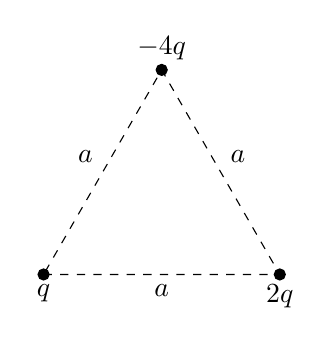
\begin{tikzpicture}
			\def\a{3};
			
			\coordinate (q) at (0,0);
			\coordinate (2q) at (0:\a);
			\coordinate(-4q) at (60:\a);
			
			\filldraw (q) circle (2pt) node [below] {$q$};
			\filldraw (2q) circle (2pt) node [below] {$2q$};
			\filldraw (-4q) circle (2pt) node [above] {$-4q$};
			
			\draw [dashed] (q) -- node [midway, below] {$a$} (2q) -- node [midway, above right] {$a$} (-4q) -- node [midway, above left] {$a$} cycle;
		\end{tikzpicture}
	\end{figure}
	The energy in the system is the amount of energy required to build the system by bringing each of the charges from infinity to its position, one by one.\\
	Let the positions of $q$, $2q$ and $-4q$ be A, B and C respectively.\\
	The energy required to bring the first charge, $q$, from infinity to A is zero, as there are no forces acting on it.\\
	The energy required to bring the second charge, $2q$, from infinity to B is 
	\begin{align*}
		U_{2q} &= - \int\limits_{\infty}^{\overrightarrow{r_\textnormal{B}}} \overrightarrow{F} \cdot \dif \overrightarrow{r}\\
		&= - \int\limits_{\infty}^{\overrightarrow{r_\textnormal{B}}} (2q) \cdot \overrightarrow{E} \cdot \dif \overrightarrow{r}\\
		&= - (2q) \int\limits_{\infty}^{\overrightarrow{r_\textnormal{B}}} \overrightarrow{E} \cdot \dif \overrightarrow{r}\\
		&= (2q) \left( \varphi(\textnormal{B}) - \varphi(\infty) \right)\\
		&= (2q) \cdot \varphi(\textnormal{B})
	\end{align*}
	where $\varphi(\textnormal{B})$ is potential at point B due to the existing charges, i.e. $q$.
	Similarly, the energy required to bring the third charge, $-4q$, from infinity to C is $(-4q) \cdot \varphi(\textnormal{C})$, where $\varphi(\textnormal{C})$ is the potential at point C due to the existing charges, i.e. $q$ and $2q$.\\
	Therefore, the total energy required is
	\begin{align*}
		U &= \left( 0 \right) + (2q) \left( \dfrac{1}{4 \pi \varepsilon_0} \dfrac{q}{a^2} \right) + (-4q) \left( \dfrac{1}{4 \pi \varepsilon_0} \dfrac{q}{a^2} + \dfrac{1}{4 \pi \varepsilon_0} \dfrac{2q}{a^2} \right)
	\end{align*}
\end{solution}

\begin{question}
	Find the potential energy in a solid sphere of charge, with charge density $\rho$ and radius $R$.
\end{question}

\begin{solution}
	Consider a solid sphere of charge with $\rho$ and $r$.
	Consider an elemental shell of thickness $\dif r$ on this sphere.\\
	Therefore,
	\begin{align*}
		\dif V &= 4 \pi r^2 \dif r\\
		\therefore \dif q &= \rho \cdot \dif V\\
		&= 4 \pi \rho r^2 \dif r
	\end{align*}
	Therefore,
	\begin{align*}
		\dif U &= \dfrac{1}{4 \pi \varepsilon_0} \dfrac{q_{\textnormal{inside}}}{r} \dif q\\
		&= \dfrac{1}{4 \pi \varepsilon_0} \dfrac{\dfrac{4}{3} \pi r^3 \rho}{r} \cdot 4 \pi r^2 \dif r \rho\\
		\therefore U &= \int\limits_{0}^{R} \dfrac{4 \pi \rho^2}{3 \varepsilon_0} r^4 \dif r\\
		&= \dfrac{4 \pi \rho^2 R^5}{15 \varepsilon_0}
	\end{align*}
\end{solution}

\section{Differential Form of Gauss' Law}

\begin{law}[Differential Form of Gauss' Law]
	\begin{equation*}
		\dif \overrightarrow{E} = \overrightarrow{\nabla} \cdot \overrightarrow{E} = \frac{\rho}{\varepsilon_0}
	\end{equation*}
	\label{Differential_Form_of_Gauss'_Law}
\end{law}

\begin{proof}
	The volume of the elemental body used for integration is denoted by $\dif^3 r$.\\
	For Cartesian coordinate systems, $\dif^3 r = \dif x \dif y \dif z$.\\
	For cylindrical coordinate systems, $\dif^3 r = r \dif \theta \dif \varphi \dif z$.\\
	For spherical coordinate systems, $\dif^3 r = r^2 \sin \theta \dif r \dif \theta \dif \varphi $.\\
	
	\begin{align*}
		\iint\limits_{\partial V} \overrightarrow{E} \cdot \dif \overrightarrow{A} &= \dfrac{1}{\varepsilon_0} Q_{\textnormal{inside}}\\
		&= \dfrac{1}{\varepsilon_0} \iiint\limits_{V} \rho \dif^3 r 
	\end{align*}
	
	If a body with volume $V$ and surface area $S$ is cut into two parts, with volumes $V_1$ and $V_2$ and surface area $S_1$ and $S_2$ respectively,
	\begin{equation*}
		V = V_1 + V_2
	\end{equation*}
	However, the surface area increases,
	\begin{equation*}
		S = S_1 + S_2 + 2 A \neq S_1 + S_2
	\end{equation*}
	where $A$ is the area of the new surface created due to the cut.\\
	Therefore,
	\begin{align*}
		\iint\limits_{S_1} \overrightarrow{E} \cdot \dif \overrightarrow{A} + \iint\limits_{S_2} \overrightarrow{E} \cdot \dif \overrightarrow{A} &= \iint\limits_{\partial V} \overrightarrow{E} \cdot \dif \overrightarrow{A}
	\end{align*}
	
	Consider a small cuboid of sides $\dif x$, $\dif y$, $\dif z$.
	Let the vertex of the cube, nearest to the origin be $(x,y,z)$.\\
	Therefore,
	\begin{align*}
		\Phi &= \quad E_z \left( x + \dfrac{\dif x}{2}, y + \dfrac{\dif y}{2}, z + \dif z \right) \dif x \dif y\\
		&\quad - E_z \left( x + \dfrac{\dif x}{2}, y + \dfrac{\dif y}{2}, z \right) \dif x \dif y\\
		&\quad + E_y \left( x + \dfrac{\dif x}{2}, y + \dif y, z + \dfrac{\dif z}{2} \right) \dif x \dif z\\
		&\quad  - E_y \left( x + \dfrac{\dif x}{2}, y, z + \dfrac{\dif z}{2} \right) \dif x \dif z\\
		&\quad + E_x \left( x + \dif x, y + \dfrac{\dif y}{2}, z + \dfrac{\dif z}{2} \right) \dif y \dif z\\
		&\quad  - E_x \left( x, y + \dfrac{\dif y}{2}, z + \dfrac{\dif z}{2} \right) \dif y \dif z\\
		&= \quad \dfrac{E_z \left( x + \dfrac{\dif x}{2}, y + \dfrac{\dif y}{2}, z + \dif z \right) - E_z \left( x + \dfrac{\dif x}{2}, y + \dfrac{\dif y}{2}, z \right)}{\dif z} \dif x \dif y\\
		&\quad + \dfrac{E_y \left( x + \dfrac{\dif x}{2}, y + \dif y, z + \dfrac{\dif z}{2} \right) - E_y \left( x + \dfrac{\dif x}{2}, y, z + \dfrac{\dif z}{2} \right)}{\dif y} \dif x \dif z\\
		&\quad + \dfrac{E_x \left( x + \dif x, y + \dfrac{\dif y}{2}, z + \dfrac{\dif z}{2} \right) - E_x \left( x, y + \dfrac{\dif y}{2}, z + \dfrac{\dif z}{2} \right)}{\dif x} \dif y \dif z\\
		&= \quad \left( \left. \dpd{E_x}{x} \right|_{\left( x + \frac{\dif x}{2}, y + \frac{\dif y}{2}, z \right)} \right.\\
		&\quad \quad + \left. \dpd{E_y}{y} \right|_{\left( x + \frac{\dif x}{2}, y, z + \frac{\dif z}{2} \right)}\\
		&\quad \quad + \left. \left. \dpd{E_z}{z} \right|_{\left( x + \frac{\dif x}{2}, y + \frac{\dif y}{2}, z \right)} \right) \dif x \dif y \dif z\\
	\end{align*}
	Therefore
	\begin{align*}
		\divergence \overrightarrow{E} &= \lim\limits_{\dif x \to 0, \dif y \to 0, \dif z \to 0} \dfrac{\Phi}{\dif x \dif y \dif z}\\
		&= \left. \left( \dpd{E_x}{x} + \dpd{E_y}{y} + \dpd{E_z}{z} \right) \right|_{(x,y,z)}\\
		&= \overrightarrow{\nabla} \cdot \overrightarrow{E}
	\end{align*}
	Therefore,
	\begin{align*}
		\overrightarrow{\nabla} \cdot \overrightarrow{E} &= \frac{\rho}{\varepsilon_0}
	\end{align*}
\end{proof}

\section{Poisson Equation}

\begin{law}[Poisson Equation]
	\begin{equation*}
		\Delta \varphi = \nabla^2 \varphi = -\frac{\rho}{\varepsilon_0}
	\end{equation*}
\end{law}

\begin{proof}
	\begin{align*}
		\overrightarrow{E} &= -\overrightarrow{\nabla} \varphi\\
		\therefore \divergence \overrightarrow{E} &= \overrightarrow{\nabla} \cdot \left( -\overrightarrow{\nabla} \varphi \right)\\
		&= -\left( \dpd[2]{\varphi}{x} + \dpd[2]{\varphi}{y} + \dpd[2]{\varphi}{x} \right)\\
		&= -\nabla^2 \varphi\\
		&= -\Delta \varphi\\
		\therefore \Delta \varphi &= -\frac{\rho}{\varepsilon_0}
	\end{align*}
\end{proof}

\begin{definition}[Laplacian]
	$\nabla^2$ is called the Laplacian.
\end{definition}

\section{Vector Analyses in Cylindrical and Spherical Coordinate Systems}

\subsection{Cylindrical Coordinates}

\begin{align*}
	\overrightarrow{\nabla} f &= \dpd{f}{r} \hat{r} + \dfrac{1}{r} \dpd{f}{\theta} \hat{\theta} + \dpd{f}{z} \hat{z}\\
	\overrightarrow{\nabla} \cdot \overrightarrow{F} &= \dfrac{1}{r} \dpd{}{r} (r F_r) + \dfrac{1}{r} \dpd{F_{\theta}}{\theta} + \dpd{F_z}{z}\\
	\overrightarrow{\nabla} \times \overrightarrow{F} &= \left( \dfrac{1}{r} \dpd{F_z}{\theta} - \dpd{F_{\theta}}{z} \right) \hat{r} + \left( \dpd{F_r}{z} - \dpd{F_z}{r} \right) \hat{\theta} + \dfrac{1}{r} \left( \dpd{}{r} (r F_{\theta}) - \dpd{F_r}{\theta} \right) \hat{z}\\
	\nabla^2 f &= \dfrac{1}{r} \dpd{}{r} \left( r \dpd{f}{r} \right) + \dfrac{1}{r^2} \dpd[2]{f}{\theta} + \dpd[2]{f}{z}
\end{align*}

\subsection{Spherical Coordinates}

\begin{align*}
	\overrightarrow{\nabla} f &= \dpd{f}{r} \hat{r} + \dfrac{1}{r} \dpd{f}{\theta} \hat{\theta} + \dfrac{1}{r \sin \theta} \dpd{f}{\varphi} \hat{\varphi}\\
	\overrightarrow{\nabla} \cdot \overrightarrow{F} &= \dfrac{1}{r^2} \dpd{}{r} (r^2 F_r) + \dfrac{1}{r \sin \theta} \dpd{}{\theta} (F_{\theta} \sin \theta) + \dfrac{1}{r \sin \theta} \dpd{F_{\varphi}}{f}\\
	\overrightarrow{\nabla} \times \overrightarrow{F} &= \quad \dfrac{1}{r \sin \theta} \left( \dpd{}{\theta} (F_{\varphi} \sin \theta) - \dpd{F_{\theta}}{\varphi} \right) \hat{r}\\
	&\quad + \dfrac{1}{r} \left( \dfrac{1}{\sin \theta} \dpd{F_r}{\varphi} - \dpd{}{r} (r F_{\varphi}) \right) \hat{\theta}\\
	&\quad + \dfrac{1}{r} \left( \dpd{}{r} (r F_{\theta}) - \dpd{F_r}{\theta} \right) \hat{\varphi}\\
	\nabla^2 f &= \dfrac{1}{r^2} \dpd{}{r} \left( r^2 \dpd{f}{r} \right) + \dfrac{1}{r^2 \sin \theta} \dpd{}{\theta} \left( \sin \theta \dpd{f}{\theta} \right) + \dfrac{1}{r^2 \sin^2 \theta} \dpd[2]{f}{\varphi}
\end{align*}

\section{Conductors}

In an electrostatic condition, the field inside a conductor is zero.
If it is not, as the conductor allows movement of charged particles, there will be a current and the condition will not be electrostatic.

\begin{question}
	A point charge $q$ is kept inside a cavity in a conducting sphere.
	Find the charge on the surfaces of the sphere.
	\begin{figure}[H]
		\begin{tikzpicture}
			\def\R{3};

			\coordinate (cavity centre) at ({(\R/4)*rand()},{(\R/4)*rand()});

			\draw (0,0) circle (\R);
			\draw (cavity centre) circle (\R/4);

			\fill (cavity centre) circle (2pt) node [left] {$q$};
		\end{tikzpicture}
	\end{figure}
\end{question}

\begin{solution}
	As the sphere is neutral, $\varphi = 0$.\\
	Therefore, $-\dfrac{\rho}{\varepsilon_0} = 0$.\\
	Therefore, by the Poisson equation,
	\begin{align*}
		\nabla^2 \varphi &= 0\\
		\therefore \dfrac{1}{r^2} \dpd{}{r} \left( r^2 \dpd{\varphi}{r} \right) &= 0\\
		\therefore \dpd{}{r} \left( r^2 \dpd{\varphi}{r} \right) &= 0\\
		\therefore r^2 \dpd{\varphi}{r} &= c\\
		\therefore \dpd{\varphi}{r} &= \dfrac{c}{r^2}\\
		\therefore \varphi &= \int \dfrac{c}{r^2} \dif r\\
		&= -\dfrac{c}{r} + d\\
		\intertext{As $\varphi(\infty) = 0$, $d = 0$. Therefore,}
		\varphi &= -\dfrac{c}{r}
	\end{align*}
	Therefore,
	\begin{align*}
		\varphi(R) = -\dfrac{c}{R}\\
		\therefore c &= -R \varphi(R)\\
		\therefore \overrightarrow{E} &= -\overrightarrow{\nabla} \varphi(r)\\
		&= -\dpd{\varphi}{r} \hat{r}\\
		&= -\left( -\dfrac{R \varphi(R)}{r^2} \right) \hat{r}\\
		&= \dfrac{R \varphi(R)}{r^2} \hat{r}
	\end{align*}
	Therefore, the field is constant all over the outer surface.\\
	Therefore, 
	\begin{align*}
		\therefore \sigma &= \dfrac{q}{4 \pi R^2}
	\end{align*}
\end{solution}

\section{Capacitors}

A capacitor is constructed by arranging two conductors, charged with opposite charges.\\
Suppose the charges on the conductors are $+Q$ and $-Q$.
Therefore,
\begin{align*}
	V &= \varphi(+) - \varphi(-)\\
	&= -\int\limits_{(-)}^{(+)} \overrightarrow{E} \cdot \dif \overrightarrow{l}\\
	&= \int\limits_{(+)}^{(-)} \overrightarrow{E} \cdot \dif \overrightarrow{l}\\
	\therefore V &\propto Q
\end{align*}

\begin{definition}[Capacitance]
	Let the charges on the opposite terminals of a capacitor be $+Q$ and $-Q$ respectively.
	The ratio between $Q$ and the potential difference between the terminals is called the capacitance of the capacitor.
	\begin{equation*}
		C = \dfrac{Q}{V}
	\end{equation*}
\end{definition}

\subsection{Parallel Plate Capacitors}

Consider a capacitor made of two conducting plates of surface area $A$ each.
Let the distance between them be $d$.
Let the charge distribution on the plates be $\sigma$ and $-\sigma$ respectively.\\
\begin{figure}[H]
	\begin{tikzpicture}
		\def\d{1};
		\def\l{3};

		\def\xMIN{-\l/2 - 1};
		\def\xMAX{\l/2 + 1};

		\def\yMIN{-1};
		\def\yMAX{\d + 1};

		\begin{scope}[lightgray, stealth-stealth]
			\draw (\xMIN,0) -- (\xMAX,0) node [right] {$y$};
			\draw (0,\yMIN) -- (0,\yMAX) node [above] {$z$};
		\end{scope}

		\begin{scope}[thick]
			\draw ({-\l/2},0) -- ({\l/2},0);
			\draw ({-\l/2},\d) -- ({\l/2},\d);
		\end{scope}
	\end{tikzpicture}
\end{figure}
If $d$ is very small compared to $A$, the plates can be considered to be infinite.\\
Therefore,
\begin{equation*}
	\overrightarrow{E} = 
		\begin{cases}
			\dfrac{\sigma}{\varepsilon_0} \hat{z} &;\quad 0 < z < d\\
			0                                     &;\quad z < 0 \text{ or } z > d\\
		\end{cases}
\end{equation*}
Therefore,
\begin{align*}
	C &= \dfrac{Q}{V}\\
	  &= \dfrac{\sigma A}{E d}\\
	  &= \dfrac{\sigma A}{\dfrac{\sigma}{\varepsilon_0} \cdot d}\\
	  &= \dfrac{A \varepsilon_0}{d}
\end{align*}

\subsection{Concentric Spherical Capacitor}

Consider a conducting sphere, with radius $R_1$ and charge $+Q$, surrounded by a concentric conducting shell of radius $R_2$ and charge $-Q$.
Therefore, the potential difference between the any point at $R_1$ from the centre and any point at $R_2$ from the centre is
\begin{align*}
	           V &= \varphi(R_1) - \varphi(R_2)\\
	             &= -\int\limits_{R_2}^{R_1} \overrightarrow{E} \cdot \dif \overrightarrow{r}\\
	             &= \int\limits_{R_1}^{R_2} \overrightarrow{E} \cdot \dif \overrightarrow{r}\\
	             &= \int\limits_{R_1}^{R_2} E \dif r\\
	             &= \int\limits_{R_1}^{R_2} \dfrac{Q}{4 \pi \varepsilon_0 r^2} \dif r\\
	             &= \left. -\dfrac{Q}{4 \pi \varepsilon_0 r} \right|_{R_1}^{R_2}\\
	             &= \dfrac{Q}{4 \pi \varepsilon_0} \left( \dfrac{1}{R_1} - \dfrac{1}{R_2} \right)\\
	\therefore C &= \dfrac{Q}{V}\\
	             &= \dfrac{4 \pi \varepsilon_0}{\dfrac{1}{R_1} - \dfrac{1}{R_2}}\\
	             &= 4 \pi \varepsilon_0 \dfrac{R_1 R_2}{R_2 - R_1}
\end{align*}

\subsection{Capacitors in Series}

\begin{figure}[H]
	\begin{circuitikz}
		\draw 
			(0,0) to             (1,0)
			(1,0) to [C = $C_1$] (3,0)
			(3,0) to             (4,0)
			(4,0) to [C = $C_2$] (6,0)
			(6,0) to             (7,0);

		\node [below left] at (2,0) {$+Q$};
		\node [below right] at (2,0) {$-Q$};
		\node [below left] at (5,0) {$+Q$};
		\node [below right] at (5,0) {$-Q$};

		\node [left] at (0,0) {$\varphi_A$};
		\node [right] at (7,0) {$\varphi_B$};
		\node [above] at (3.5,0) {$\varphi_C$};
	\end{circuitikz}
\end{figure}

\begin{align*}
	           V                              &= (\varphi_A - \varphi_C) + (\varphi_C - \varphi_B)\\
	                                          &= \dfrac{Q}{C_1} + \dfrac{Q}{C_2}\\
	\therefore \dfrac{Q}{C_{\textnormal{eq}}} &= \dfrac{Q}{C_1} + \dfrac{Q}{C_2}\\
	\therefore \dfrac{1}{C_{\textnormal{eq}}} &= \dfrac{1}{C_1} + \dfrac{1}{C_2}
\end{align*}

\subsection{Capacitors in Parallel}

\begin{align*}
	C_{\textnormal{eq}} &= C_1 +C_2
\end{align*}

\subsection{Energy Stored in a Capacitor}

Consider a capacitor with potential difference $V$ and charge $Q$.\\
The energy required to move an elemental charge $\dif q$ from the negatively charged plate to the positively charged plate is
\begin{align*}
	           \dif U &= V \dif q\\
	                  &= \dfrac{q}{C} \dif q\\
	\therefore U      &= \int\limits_{0}^{Q} \dfrac{q}{C} \dif q\\
	                  &= \dfrac{Q^2}{2 C}\\
			  &= \dfrac{1}{2} Q V\\
			  &= \dfrac{1}{2} C V^2
\end{align*}

\subsection{Energy Density}

Consider a parallel plate capacitor, with plates of area $A$, with distance $d$ between them and charge $+Q$ and $-Q$ respectively.
The electric field between them is
\begin{align*}
	E                                     & = \dfrac{\sigma}{\varepsilon_0} \\
                                              & = \dfrac{Q}{\varepsilon_0 A}    \\
	\therefore E d                        & = \dfrac{Q d}{\varepsilon_0 A}  \\
	\intertext{As $V = E d$,}
	V                                     & = \dfrac{Q d}{\varepsilon_0 A}  \\
	\therefore \dfrac{A \varepsilon_0}{d} & = \dfrac{Q}{V}                  \\
	\therefore \dfrac{A \varepsilon_0}{d} & = C
\end{align*}
Therefore,
\begin{align*}
	U                         & = \dfrac{1}{2} C V^2                              \\
                                  & = \dfrac{1}{2} \varepsilon_0 \dfrac{A}{d} E^2 d^2 \\
                                  & = \dfrac{1}{2} (A d) \varepsilon_0 E^2            \\
	\therefore \dfrac{U}{A d} & = \dfrac{1}{2} \varepsilon_0 E^2                  \\
	\intertext{Therefore, as $A d$ is the volume of the space between the plates of the capacitor, $\dfrac{U}{A d}$ is called the energy density. Therefore,}
	u                         & = \dfrac{1}{2} \varepsilon_0 E^2
\end{align*}

In general, for a charged body with volume charge density $\rho$, assuming $\varphi(\infty) = 0$,
\begin{align*}
	U & = \iiint\limits_{V} \dfrac{1}{2} \rho \varphi \dif^3 r \\
	\intertext{As $\rho = -\varepsilon_0 \nabla^2 \varphi$,}
	U & = \iiint\limits_{V} \dfrac{1}{2} (-\varepsilon_0 \nabla^2 \varphi) \varphi \dif^3 r
\end{align*}
\begin{align*}
	\overrightarrow{E}                                 & = -\overrightarrow{\nabla} \varphi                                                     \\
	\therefore \nabla^2 \varphi                        & = \overrightarrow{\nabla} \cdot \left( \overrightarrow{\nabla} \varphi \right)         \\
	\therefore \left( \nabla^2 \varphi \right) \varphi & = \overrightarrow{\nabla} \cdot \left( \overrightarrow{\nabla} \varphi \right) \varphi \\
\end{align*}
\begin{align*}
	\overrightarrow{\nabla} \cdot \left( \varphi \left( \overrightarrow{\nabla} \varphi \right) \right) & = \left( \overrightarrow{\nabla} \varphi \right) \left( \overrightarrow{\nabla} \varphi \right) + \varphi \overrightarrow{\nabla} \cdot \left( \overrightarrow{\nabla} \varphi \right) \\
                                                                                                            & = \left( -\overrightarrow{E} \right) \left( -\overrightarrow{E} \right) + \varphi \nabla^2 \varphi                                                                                     \\
	\therefore \nabla^2 \varphi                                                                         & = \overrightarrow{\nabla} \cdot \left( -\varphi \overrightarrow{E} \right) - E^2
\end{align*}
Therefore, substituting in $U$,
\begin{align*}
	U            & = \iiint\limits_{V} \left( -\dfrac{1}{2} \varepsilon_0 \right) \left( \overrightarrow{\nabla} \cdot \left( -\varphi \overrightarrow{E} \right) - E^2 \right) \dif^3 r                       \\
                     & = \dfrac{1}{2} \varepsilon_0 \iiint\limits_{V} \overrightarrow{\nabla} \cdot \left( \varphi \overrightarrow{E} \right) \dif^3 r + \iiint\limits_{V} \dfrac{1}{2} \varepsilon_0 E^2 \dif^3 r \\
                     & = \dfrac{1}{2} \varepsilon_0 \iint\limits_{\partial V} \varphi \overrightarrow{E} \cdot \dif \overrightarrow{A} + \iiint\limits_{V} \dfrac{1}{2} \varepsilon_0 E^2 \dif^3 r                 \\
	\intertext{As there are no charges at infinity, the electric field at infinity is zero. Therefore, the flux through the large surface is zero. Therefore, $\varepsilon_0 \iint\limits_{\partial V} \varphi \overrightarrow{E} \cdot \dif \overrightarrow{A} = 0$. Also, according to the initial assumption, $\varphi(\infty) = 0$.}
	\therefore U & = \iiint\limits_{V} \dfrac{1}{2} \varepsilon_0 E^2 \dif^3 r                                                                                                                                 \\
	\therefore u & = \dfrac{1}{2} \varepsilon_0 E^2
\end{align*}

\begin{question}
	Find the potential energy contained in a sphere of charge with radius $R$.
\end{question}

\begin{solution}
	\begin{align*}
		E &= 
			\begin{cases}
				\dfrac{\rho r}{3 \varepsilon_0}                            & ;\quad r < R \\
				\dfrac{\dfrac{4}{3} \pi R^3 \rho}{4 \pi \varepsilon_0 r^2} & ;\quad r > R \\
			\end{cases}
	\end{align*}
	Therefore
	\begin{align*}
		U & = \iiint\limits_{V} \dfrac{1}{2} \varepsilon_0 E^2 \dif^3 r                                                                                                                                                                                          \\
                  & = \int\limits_{0}^{R} \dfrac{1}{2} \varepsilon_0 \left( \dfrac{\rho r}{3 \varepsilon_0} \right)^2 \cdot 4 \pi r^2 \dif r + \int\limits_{R}^{\infty} \dfrac{1}{2} \varepsilon_0 \left( \dfrac{R^3 \rho}{3 \varepsilon_0 r^2} \right) 4 \pi r^2 \dif r \\
                  & = \dfrac{2 \pi \rho^2}{9 \varepsilon_0} \int\limits_{0}^{R} r^4 \dif r + \dfrac{2 \pi \rho^2 R^6}{9 \varepsilon_0} \int\limits_{R}^{\infty} \dfrac{1}{r^2} \dif r                                                                                    \\
                  & = \dfrac{2 \pi \rho^2}{9 \varepsilon_0} \left( \dfrac{R^5}{5} \right) + \dfrac{2 \pi \rho^2 R^6}{9 \varepsilon_0} \left. \left( -\dfrac{1}{r} \right) \right|_{R}^{\infty}                                                                           \\
                  & = \dfrac{2 \pi \rho^2 R^5}{9 \varepsilon_0} \left( \dfrac{1}{5} + 1 \right)                                                                                                                                                                          \\
                  & = \dfrac{2 \pi \rho^2 R^5}{9 \varepsilon_0} \cdot \dfrac{6}{5}                                                                                                                                                                                       \\
                  & = \dfrac{4 \pi \rho^2 R^5}{15 \varepsilon_0}
	\end{align*}
\end{solution}

\section{Dielectric Materials}

\begin{definition}[Dielectric constant or relative permittivity]
	If the electric field in a dielectric material across some voltage and some distance is $E$, and the electric field in an identical setup, with a vacuum is $E_0$, the ratio between $E_0$ and $E$ is called the dielectric constant of the material or the relative permittivity of the material.
	\begin{equation*}
		\kappa_E = \dfrac{E_0}{E}
	\end{equation*}
\end{definition}

Consider a parallel plate capacitor with a dielectric slab of $\kappa_E$ inserted between its plates.\\
Let the surface charge densities on each of the plates be $+\sigma_{\textnormal{free}}$ and $-\sigma_{\textnormal{free}}$, and charges $+Q$ and $-Q$.\\
Let the field inside the capacitor, if it the dielectric slab is absent, be $E_0$, and the field inside the capacitor, if the dielectric slab is present be $E$.\\
Consider a cuboid Gaussian surface at the interface of the dielectric slab and the plate with charge density $+\sigma_{\textnormal{free}}$.\\
As the electric field entering the Gaussian surface is more than the electric field exiting it, there must be some negative charge on the interface.\\
Let the surface charge density of this bound charge be $-\sigma_{\textnormal{bound}}$.\\
Therefore, the net field inside the capacitor is
\begin{equation*}
	E = \dfrac{\sigma_{\textnormal{free}} - \sigma_{\textnormal{bound}}}{\varepsilon_0}
\end{equation*}

\begin{definition}[Permittivity of a dielectric]
	\begin{align*}
		\dfrac{C}{C_0} & = \dfrac{\dfrac{Q}{V}}{\dfrac{Q}{V_0}} \\
                               & = \dfrac{V_0}{V}                       \\
                               & = \dfrac{E_0 d}{E d}                   \\
                               & = \dfrac{E_0}{E}                       \\
                               & = \kappa_E                             \\
		\therefore C   & = C_0 \kappa_E                         \\
                               & = \varepsilon_0 \kappa_E \dfrac{A}{d}
	\end{align*}
	$\varepsilon = \varepsilon_0 \kappa_E$ is called the permittivity of the dielectric.
\end{definition}

\subsection{Gauss' Law in Dielectric Materials}

\begin{align*}
	\iint \overrightarrow{E_0} \cdot \dif \overrightarrow{A}                                 & = \dfrac{Q_{\textnormal{free}}}{\varepsilon_0} \\
	\therefore \iint \kappa_E \overrightarrow{E} \cdot \dif \overrightarrow{A}               & = \dfrac{Q_{\textnormal{free}}}{\varepsilon_0} \\
	\therefore \iint \kappa_E \varepsilon_0 \overrightarrow{E} \cdot \dif \overrightarrow{A} & = Q_{\textnormal{free}}
\end{align*}

\begin{definition}[Electric displacement field]
	\begin{equation*}
		\overrightarrow{D} = \varepsilon_0 \kappa_E \overrightarrow{E} = \varepsilon \overrightarrow{E}
	\end{equation*}
	is called the electric displacement field.
\end{definition}

Therefore,
\begin{align*}
	\iint\limits_{\partial V} \overrightarrow{D} \cdot \dif \overrightarrow{A}             & = Q_{\textnormal{free}}    \\
	\therefore \iiint\limits_{V} \overrightarrow{\nabla} \cdot \overrightarrow{D} \dif^3 r & = \rho_{\textnormal{free}} \\
	\therefore \overrightarrow{\nabla} \cdot \overrightarrow{D}                            & = \rho_{\textnormal{free}}
\end{align*}

\begin{question}
	A slab of dielectric material, with thickness $x$ is inserted in a parallel plate capacitor, with plates of surface area $A$ and distance $d$ between them, as shown.
	\begin{figure}[H]
		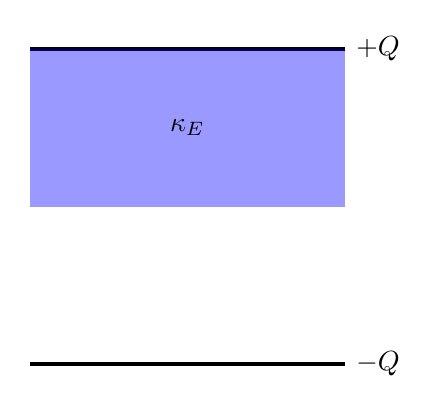
\begin{tikzpicture}
			\def\d{4};
			\def\x{2};
			\def\l{4};

			\begin{scope}[ultra thick]
				\draw (-\l/2,0) -- (\l/2,0) node [right] {$-Q$};
				\draw (-\l/2,\d) -- (\l/2,\d) node [right] {$+Q$};
			\end{scope}

			\begin{scope}
				\fill [blue, opacity = 0.4] (-\l/2,\d) rectangle (\l/2,\d-\x);
				\node at (0,\d-\x/2) {$\kappa_E$};
			\end{scope}
		\end{tikzpicture}
	\end{figure}
	Find the charge density on the interface of the dielectric slab and the effective capacitance.
\end{question}

\begin{solution}
	As the charge on the plates is $+Q$ and $-Q$ respectively, and as the area of the plates is $A$,
	\begin{align*}
		\sigma_{\textnormal{free}} & = \dfrac{Q}{A}
	\end{align*}
	Consider a cuboid Gaussian surface at the interface the dielectric slab and the free space, inside the capacitor.
	As the field entering the Gaussian surface is less than the field exiting it, there must a bound positive charge at the interface.
	Let the surface charge density of this bound charge be $+\sigma_b$.
	\begin{align*}
		E_2 S - E_1 S                                                               & = \dfrac{\sigma_b A}{\varepsilon_0}                   \\
		\therefore \dfrac{Q}{\varepsilon_0 A} - \dfrac{Q}{\varepsilon_0 \kappa_E A} & = \dfrac{\sigma_b}{\varepsilon_0}                     \\
		\therefore \sigma_b                                                         & = \dfrac{Q}{A} \left( 1 - \dfrac{1}{\kappa_E} \right) \\
                                                                                            & = \dfrac{Q}{A} \cdot \dfrac{\kappa_E - 1}{\kappa_E}   \\
		\therefore \sigma_b                                                         & \le \sigma_{\textnormal{free}}
	\end{align*}
	~\\
	\begin{align*}
		C & = \dfrac{Q}{V}                                                                                                   \\
                  & = \dfrac{Q}{E_1 x + E_2 (d - x)}                                                                                 \\
                  & = \dfrac{\cancel{Q}}{\dfrac{\cancel{Q}}{\varepsilon_0 \kappa A} x + \dfrac{\cancel{Q}}{\varepsilon_0 A} (d - x)} \\
                  & = \dfrac{\varepsilon_0 A}{\dfrac{x}{k} + d - x}                                                                  \\
                  & = \varepsilon_0 \dfrac{A}{d - x \left( 1 - \dfrac{1}{k} \right)}
	\end{align*}
\end{solution}

\newpage
\part{Electrodynamics}

\section{Currents}

\begin{definition}[Current]
	Current is defined as the rate of charge passing through a cross-sectional area.
	\begin{equation*}
		I = \dod{q}{t}
	\end{equation*}
\end{definition}

\begin{definition}[Current density]
	\begin{equation*}
		\overrightarrow{J} = \dfrac{I}{A}
	\end{equation*}
	$\overrightarrow{J}$ is called the current density.\\
	Therefore, the current is the flux of $\overrightarrow{J}$.
\end{definition}

\subsection{Continuity Law}

\begin{align*}
	Q                     & = \iiint\limits_{V} \rho(x,y,z,t) \dif^3 r           \\
	\therefore \dod{Q}{t} & = \dod{}{t} \iiint\limits_{V} \rho(x,y,z,t) \dif^3 r \\
                              & = \iiint\limits_{V} \dod{\rho}{t} \dif^3 r
\end{align*}
\begin{align*}
	I & = \iint\limits_{\partial V} \overrightarrow{J} \dif \overrightarrow{a}
\end{align*}
\begin{align*}
	I                                                                                     & = - \dod{Q}{t}                              \\
	\therefore \iint\limits_{\partial V} \overrightarrow{J} \cdot \dif \overrightarrow{A} & = \iiint\limits_{V} -\dpd{\rho}{t} \dif^3 r \\
	\intertext{Therefore, by the divergence theorem,}
	\iiint\limits_{V} \overrightarrow{\nabla} \cdot \overrightarrow{J} \dif^3 r           & = \iiint\limits_{V} -\dpd{\rho}{t} \dif^3 r \\
	\therefore \overrightarrow{\nabla} \cdot \overrightarrow{J}                           & = -\dpd{\rho}{t}
\end{align*}

\subsection{Charge Carriers}

Current density is the product of the total charge and the net drift velocity of the charge carriers.
\begin{align*}
	\overrightarrow{J} & = n q \overrightarrow{v_{\textnormal{drift}}}
\end{align*}
where $n$ is the number of charge carriers and $q$ is the charge on each of them.
\begin{align*}
	\overrightarrow{v_{\textnormal{drift}}} & = \frac{1}{n} \sum \overrightarrow{v_i}
\end{align*}
where $\overrightarrow{v_i}$ is the velocity of the $i^{\text{th}}$ charge carrier.

\section{Ohm's Law}

\begin{law}[Ohm's Law]
	The voltage across two points on a conductor is directly proportional to the current through the conductor.
	The constant of proportionality is called the resistance of the conductor.
	\begin{equation*}
		\frac{V}{I} = R
	\end{equation*}
	\label{Ohm's_Law}
\end{law}

\section{Resistors}

\subsection{Resistivity}

Consider a conductor of cross-sectional area $A$ and length $L$ connected to a potential difference of $V$.
Let the current passing through it be $I$.\\
Therefore,
\begin{align*}
	I & = J A \\
	V & = E L
\end{align*}
Therefore,
\begin{align*}
	R & = \frac{V}{I}          \\
          & = \frac{E L}{J A}      \\
	\intertext{As $E \propto J$, $E$ can be written as $\rho J$. Therefore,}
	R & = \frac{\rho J L}{J A} \\
          & = \rho \frac{L}{A}
\end{align*}

\begin{definition}[Resistivity]
	If
	\begin{equation*}
		R = \rho \frac{L}{A}
	\end{equation*}
	$\rho$ is called the resistivity of the conductor.\\
	$\sigma = \frac{1}{\rho}$ is called the conductivity of the conductor.\\
	They are constant for a particular material.
\end{definition}

\subsection{Resistors in Series}

\begin{figure}[H]
	\begin{circuitikz}
		\draw (0,0) to [R = $R_1$, i = $I$] (2,0) to [R = $R_2$] (4,0);
	\end{circuitikz}
\end{figure}
Let $V_1$ and $V_2$ be the voltages across $R_1$ and $R_2$ respectively.\\
As the resistors are in series,
\begin{align*}
	V & = V_1 + V_2     \\
          & = I R_1 + I R_2 \\
          & = I (R_1 + R_2) \\
          & = I R_{\textnormal{equivalent}}
\end{align*}
Therefore,
\begin{align*}
	R_{\textnormal{equivalent}} & = R_1 + R_2
\end{align*}

\subsection{Resistors in Parallel}

\begin{figure}[H]
	\begin{circuitikz}
		\draw (0,0) -- (1,0);
		\draw (1,0) to (2,1) to [R = $R_1$] (4,1) to (5,0);
		\draw (1,0) to (2,-1) to [R = $R_2$] (4,-1) to (5,0);
		\draw (5,0) -- (6,0);
	\end{circuitikz}
\end{figure}
Let $I_1$ and $I_2$ be the currents through $R_1$ and $R_2$ respectively.\\
As the resistors are in parallel,
\begin{align*}
	I & = I_1 + I_2                                      \\
          & = \frac{V}{R_1} + \frac{V}{R_2}                  \\
          & = V \left( \frac{1}{R_1} + \frac{1}{R_2} \right) \\
          & = \frac{V}{R_{\textnormal{equivalent}}}
\end{align*}
Therefore,
\begin{align*}
	\frac{1}{R_{\textnormal{equivalent}}} & = \frac{1}{R_1} + \frac{1}{R_2}
\end{align*}

\section{Power and Energy}

Consider a resistor of resistance $R$ connected to a source of voltage $V$.\\
The energy needed to transfer a charge $\dif q$ across $V$ is
\begin{align*}
	\dif U & = V \dif q
\end{align*}
Therefore the power dissipated across the resistor is
\begin{align*}
	P & = \dod{U}{t}   \\
          & = V \dod{q}{t} \\
          & = V I          \\
          & = I^2 R
\end{align*}

\section{RC Series Circuit}

\begin{figure}[H]
	\begin{circuitikz}
		\draw 
			(0,0) to [short, i = $I(t)$] (0,2)
			(0,2) to [R = $R$] (3,2)
			(3,2) to [C = $C$] (3,0)
			(3,0) to [battery1 = $\varepsilon$] (0,0);
	\end{circuitikz}
\end{figure}

\subsection{Charge on the Capacitor}

\begin{align*}
	\oint \overrightarrow{E} \cdot \overrightarrow{\dif l} & = 0                                                                                                \\
	\therefore -\varepsilon + I R + \frac{Q}{C}            & = 0                                                                                                \\
	\therefore I R + \frac{Q}{C}                           & = \varepsilon                                                                                      \\
	\therefore I + \frac{Q}{R C}                           & = \frac{\varepsilon}{R}                                                                            \\
	\therefore \dod{q}{t} + \frac{1}{R C} Q                & = \frac{\varepsilon}{R}                                                                            \\
	\therefore Q                                           & = \frac{1}{e^{\int \frac{1}{R C} \dif t}} \int e^{\int \frac{1}{R C} \dif t} \frac{\varepsilon}{R} \\
                                                               & = \frac{1}{e^{\frac{t}{R C}}} \varepsilon C e^{\frac{t}{R C}} + D
\end{align*}
As $Q(t = 0) = 0$, $D = -\varepsilon C$.\\
Therefore,
\begin{align*}
	Q & = \varepsilon C \left( 1 - e^{-\frac{t}{R C}} \right)
\end{align*}

\begin{definition}[Time constant of RC circuit]
	$\tau = R C$ is called the time constant of a circuit with a resistor of resistance $R$ and a capacitor of capacitance $C$ connected in series.
\end{definition}

\subsection{Current in the Circuit}

\begin{align*}
	I & = \dod{Q}{t} \\
          & = \frac{\varepsilon}{R} e^{-\frac{t}{R C}}
\end{align*}

\subsection{Power and Energy}

The power supplied by the battery is
\begin{align*}
	P_{\varepsilon} & = \varepsilon I \\
                        & = \frac{\varepsilon^2}{R} e^{-\frac{t}{R C}}
\end{align*}
The power dissipated at the resistor is
\begin{align*}
	P_R & = I^2 R \\
            & = \frac{\varepsilon^2}{R} e^{-\frac{2 t}{R C}}
\end{align*}
The energy stored in the capacitor is
\begin{align*}
	U_C & = \frac{Q^2}{2 C} \\
            & = \frac{\varepsilon^2 C}{2} \left( 1 - e^{-\frac{t}{R C}} \right)^2
\end{align*}
Therefore the power in the capacitor is
\begin{align*}
	P_C & = \dod{U_C}{t}                                                                         \\
            & = \varepsilon^2 C \left( 1 - e^{-\frac{t}{R C}} \right) \frac{e^{-\frac{t}{R C}}}{R C} \\
            & = \frac{\varepsilon^2}{R} e^{-\frac{2 t}{R C}}
\end{align*}
Therefore,
\begin{align*}
	P_{\varepsilon} & = P_R + P_C
\end{align*}
Therefore, the power is conserved.

\begin{question}
	A thick conducting, cylindrical shell with inner radius $a$, outer radius $b$, and height $h$ is charged with conductivity $\sigma(r) = \alpha r^2$.
	Assuming $h << a$,
	\begin{enumerate}
		\item Find the net resistance if the flat faces are connected to terminals of a battery.
		\item Find the net resistance if the inner and outer surfaces are connected to terminals of a battery.
	\end{enumerate}
\end{question}

\begin{solution}
	\begin{enumerate}[leftmargin = *]
		\item
			Consider an elemental resistor, i.e. a thin cylindrical shell of radius $a < r < b$ and thickness $\dif r$.\\
			Therefore,
			\begin{align*}
				\dif R & = \frac{1}{\sigma} \frac{L}{A}                  \\
                                       & = \frac{1}{\alpha r^2} \frac{h}{2 \pi r \dif r} \\
                                       & = \frac{h}{2 \pi \alpha r^3 \dif r}
			\end{align*}
			As the elemental resistors are connected in parallel,
			\begin{align*}
				\frac{1}{R}  & = \int \frac{1}{\dif R}                                 \\
                                             & = \int\limits_{a}^{b} \frac{2 \pi \alpha r^3 \dif r}{h} \\
                                             & = \frac{\pi \alpha}{2 h} (b^4 - a^4)                    \\
				\therefore R & = \frac{2 h}{\pi \alpha (b^4 - a^4)}
			\end{align*}
			~\\
			Alternatively,
			\begin{align*}
				J & = \sigma E               \\
                                  & = \sigma \frac{V}{h}     \\
                                  & = \alpha r^2 \frac{V}{h} \\
			\end{align*}
			\begin{align*}
				I & = \iint \overrightarrow{J} \cdot \overrightarrow{\dif A}          \\
                                  & = \int\limits_{a}^{b} \alpha r^2 \frac{V}{h} \cdot 2 \pi r \dif r \\
                                  & = \frac{\pi \alpha}{2 h}(b^4 - a^4) V
			\end{align*}
			Therefore,
			\begin{align*}
				R & = \frac{V}{I} \\
                                  & = \frac{2 h}{\pi \alpha (b^4 - a^4)}
			\end{align*}
			~\\
			The charge density in the body is
			\begin{align*}
				\varrho &= \varepsilon_0 \overrightarrow{\nabla} \cdot \overrightarrow{E}\\
				&= 0
			\end{align*}
		\item
			Consider an elemental resistor, i.e. a thin cylindrical shell of radius $a < r < b$ and thickness $\dif r$.\\
			Therefore,
			\begin{align*}
				\dif R & = \frac{1}{\sigma} \frac{L}{A}                  \\
                                       & = \frac{1}{\alpha r^2} \frac{\dif r}{2 \pi r h} \\
                                       & = \frac{\dif r}{2 \pi \alpha r^3 h}
			\end{align*}
			As the elemental resistors are connected in series,
			\begin{align*}
				R & = \int \dif R                                                                \\
                                  & = \int\limits_{a}^{b} \frac{\dif r}{2 \pi \alpha r^3 h}                      \\
                                  & = \frac{1}{2 \pi \alpha h} \left( -\frac{1}{2 b^2} + \frac{1}{2 a^2} \right) \\
                                  & = \frac{1}{4 \pi \alpha h} \left( \frac{1}{a^2} - \frac{1}{b^2} \right)
			\end{align*}
			~\\
			Alternatively,
			\begin{align*}
				J &= \sigma E\\
				\therefore \frac{I}{2 \pi r h} &= \alpha r^2 E\\
				\therefore E &= \frac{I}{2 \pi \alpha r^3 h}
			\end{align*}
			Therefore,
			\begin{align*}
				V &= \int\limits_{a}^{b} E \dif r\\
				&= \int\limits_{a}^{b} \frac{I \dif r}{2 \pi \alpha r^3 h} \left( \frac{1}{a^2} - \frac{1}{b^2} \right)
			\end{align*}
			Therefore,
			\begin{align*}
				R &= \frac{V}{I}\\
				&= \frac{1}{4 \pi \alpha h} \left( \frac{1}{a^2} - \frac{1}{b^2} \right)
			\end{align*}
			~\\
			The charge density in the body is
			\begin{align*}
				\varrho &= \varepsilon_0 \overrightarrow{\nabla} \cdot \overrightarrow{E}\\
				&= \varepsilon_0 \frac{1}{r} \dod{}{r} (r E_r)\\
				&= \varepsilon_0 \frac{1}{r} \dod{}{r} \left( \frac{I}{2 \pi \alpha r^3 h} \right)\\
				&= -\frac{\varepsilon_0 I}{\pi \alpha r^4 h}
			\end{align*}
			Therefore, the charge in the body is not zero.\\
			However, it is constant in time.
			Therefore, in the steady state, it does not violate Kirchoff's Current Law.\\
			Consider a cuboid Gaussian surface which contains part of the elemental ring in it.\\
			As $\sigma$ is varying, the electric field decreases as $r$ increases.\\
			Therefore by Gauss' Law, as the electric field entering the Gaussian surface is more than the electric field exiting the Gaussian surface.
			Hence, there must be a negative charge inside the Gaussian surface.
	\end{enumerate}
\end{solution}

\newpage
\part{Magnetism}

\section{Magnetic Force}

\begin{law}
	\begin{equation*}
		\dif \overrightarrow{F} = I \overrightarrow{\dif l} \times \overrightarrow{B}
	\end{equation*}
\end{law}
Consider a stream of charged particles moving with velocity $\overrightarrow{v}$.
Therefore, $\dif l = v \dif t$.\\
Therefore,
\begin{align*}
	\dif \overrightarrow{F} & = I \overrightarrow{\dif l} \times \overrightarrow{B}               \\
                                & = \dod{q}{t} ( \overrightarrow{v} \dif t) \times \overrightarrow{B} \\
                                & = \dif q \overrightarrow{v} \times \overrightarrow{B}
\end{align*}

\section{Lorentz Force}

\begin{definition}[Lorentz force]
	The net force due to the electric field and due to the magnetic field is acting on a charged particle is called the Lorentz force.
	\begin{equation*}
		\overrightarrow{F} = q \overrightarrow{E} + q \overrightarrow{v} \times \overrightarrow{B}
	\end{equation*}
\end{definition}
This force is dependent on the velocity of the charge.
Therefore, the force will change depending on the frame of reference.
Therefore it apparently violates the basic assumption that interactions between bodies are the same irrespective of the frame of reference.

\begin{question}
	A charged particle of charge $q$ and mass $m$ enters a region with uniform magnetic field as shown.
	\begin{figure}[H]
		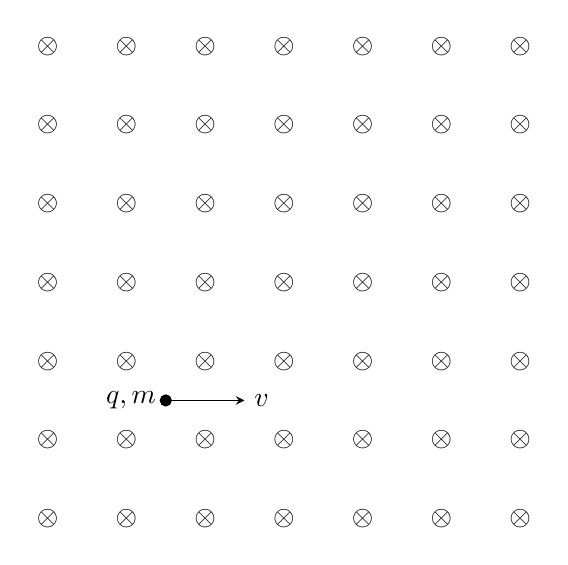
\begin{tikzpicture}
			\def\F{1};

			\foreach \x in {-1.5,...,4.5}
			{
				\foreach \y in {-1.5,...,4.5}
				{
					\node at (\x,\y) {$\otimes$};
				}
			}

			\filldraw (0,0) circle (2pt) node [left] {$q, m$};

			\begin{scope}[-stealth]
				\draw (0,0) -- ++(0:\F) node [right] {$v$};
			\end{scope}
		\end{tikzpicture}
	\end{figure}
	How will the particle move?
\end{question}

\begin{solution}
	The force is perpendicular to $\overrightarrow{v}$ and $\overrightarrow{B}$.
	\begin{figure}[H]
		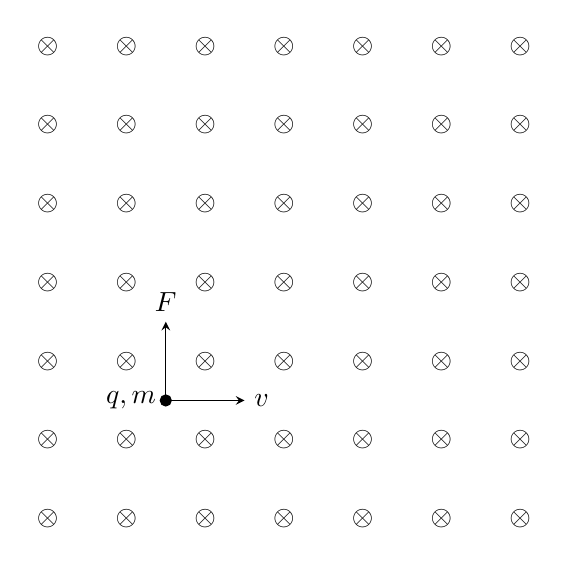
\begin{tikzpicture}
			\def\F{1};

			\foreach \x in {-1.5,...,4.5}
			{
				\foreach \y in {-1.5,...,4.5}
				{
					\node at (\x,\y) {$\otimes$};
				}
			}

			\filldraw (0,0) circle (2pt) node [left] {$q, m$};

			\begin{scope}[-stealth]
				\draw (0,0) -- ++(0:\F) node [right] {$v$};
				\draw (0,0) -- ++(90:\F) node [above] {$F$};
			\end{scope}
		\end{tikzpicture}
	\end{figure}
	Therefore, as the force is always perpendicular to the velocity, it will change the direction of the velocity and not its magnitude.
	Therefore, the particle will move in a circle.\\
	\begin{align*}
		F            & = q v B           \\
                             & = \frac{m v^2}{R} \\
		\therefore R & = \frac{m v}{q B}
	\end{align*}
\end{solution}

\subsection{Cyclotron}

A cyclotron is a setup used to accelerate charged particles.
It is constructed with regions of magnetic field $\overrightarrow{B}$ and regions of electric field $\overrightarrow{E}$ as shown.
\begin{figure}[H]
	\begin{tikzpicture}
		\def\R{4};
		\def\d{2};
		\def\l{0.5};
	
		\begin{scope}[red]
			\draw (\R + 2,\d/2) arc (0:180:\R + 2);
			\draw (-\R - 2,\d/2) -- (\R + 2,\d/2);
	
			\draw (-\R - 2,-\d/2) arc (180:360:\R + 2);
			\draw (-\R - 2,-\d/2) -- (\R + 2,-\d/2);
		\end{scope}
	
		\filldraw ($ (\l,-\d/2) + (0,2pt) $) circle (2pt);
	
		\coordinate (particle) at ($ (\l,-\d/2) + (0,2pt) $);
	
		\foreach \r in {1,3}
		{
			\draw (particle) -- ++(0,\d);
	
			\draw ($ (particle) + (0,\d) $) arc (0:180:\r);
			
			\draw ($ (particle) + (0,\d) + (-2*\r,0) $) -- ++(0,-\d);
	
			\draw ($ (particle) + (0,\d) + (-2*\r,0) + (0,-\d) $) arc (180:360:\r + 1);
	
			\coordinate (particle) at ($ (particle) + (\r + 1,0) $);
		}
	\end{tikzpicture}
\end{figure}
The semicircular areas have magnetic field $\overrightarrow{B}$ directed inwards and the region between the semicircular areas have $\overrightarrow{E}$ directed upwards.
The electric field changes directions such that the frequency of the field is half the frequency of the rotation of the charged particle.\\
The particle with mass $m$ and charge $q$ starts as shown and is accelerated under the electric field till it enters the semicircular area.\\
Let the velocity of the particle when it enters the semicircular area be $v_0$.
It goes in a semicircle of radius $\frac{m v_0}{q B}$ and again enters the region with $\overrightarrow{E}$.\\
This process is continued till the particle is ejected.

\section{Thompson's Experiment}

Electrons from a cathode ray tube are accelerated under $\overrightarrow{E}$ in the first region.
When they enter the region with the magnetic field, they move in a circle.
\begin{align*}
	e E                    & = e v B                     \\
	\therefore v           & = \frac{E}{B}               \\
	\therefore R           & = \frac{m v}{e B}           \\
                               & = \frac{m \frac{E}{B}}{q B} \\
                               & = \frac{m E}{e B^2}         \\
	\therefore \frac{e}{m} & = \frac{E}{R B^2}
\end{align*}
Therefore, $\frac{e}{m}$ can be physically calculated.

\section{Biot-Savart Law}

\begin{law}[Biot-Savart Law]
	\begin{align*}
		\dif \overrightarrow{B} & = \frac{\mu_0}{4 \pi} \frac{I \dif \overrightarrow{l} \times \hat{r}}{r^2} \\
		\therefore B            & = \frac{\mu_0}{4 \pi} \frac{q \overrightarrow{v} \times \hat{r}}{r^2}
	\end{align*}
	\label{Biot-Savart_Law}
\end{law}

\begin{question}
	Find the magnetic field due on the axis of a ring of radius $R$ carrying current $I$.
	\begin{figure}[H]
		\begin{tikzpicture}
			\def\R{2};
			\def\z{4};

			\draw (0,0) circle [x radius = \R, y radius = 0.4*\R];

			\draw [dashed] (0,0) -- (0,\z) node[midway, right] {$z$};
			\draw [dashed] (0,0) -- (\R,0) node[midway, below] {$R$};
		\end{tikzpicture}
	\end{figure}
\end{question}

\begin{solution}
	\begin{figure}[H]
		\begin{tikzpicture}
			\def\R{2};
			\def\z{4};
			\def\F{1};

			\begin{scope}[dashed]
				\draw (-\R,0) -- (0,0) node [midway, below] {$R$};
				\draw (0,0) -- (\R,0) node [midway, below] {$R$};

				\draw (0,0) -- (0,\z) node [midway, left] {$z$};
			\end{scope}

			\begin{scope}
				\node at (-\R,0) {$\odot$};
				\node at (\R,0) {$\otimes$};
			\end{scope}

			\begin{scope}[dashed, blue]
				\draw (-\R,0) -- (0,\z);
				\draw (\R,0) -- (0,\z);
			\end{scope}

			\begin{scope}[red, -stealth]
				\draw (0,\z) -- ($ (0,\z)!1cm!90:(\R,0) $);
				\draw (0,\z) -- ($ (0,\z)!1cm!-90:(-\R,0) $);
			\end{scope}
		\end{tikzpicture}
	\end{figure}
	Due to symmetry of the ring, the components of the differential fields in the $z$ direction are added up and all others are cancelled out.\\
	Therefore,
	\begin{align*}
		\overrightarrow{B} & = \hat{z} \int \dif B \cos(90 - \theta)                                                                       \\
                                   & = \hat{z} \int\limits_{0}^{2 \pi R} \frac{\mu_0}{4 \pi} \frac{I \dif l}{z^2 + R^2} \frac{R}{\sqrt{R^2 + z^2}} \\
                                   & = \frac{\mu_0}{4 \pi} \frac{I R^2}{\left( z^2 + R^2 \right)^{\frac{3}{2}}} \hat{z}
	\end{align*}
\end{solution}

\begin{question}
	Find the magnetic field at a distance $r$ from an infinite wire carrying current $I$.
\end{question}

\begin{solution}
	Consider an elemental current carrier of length $\dif z$ at a distance $z$ from the origin.\\
	Therefore,
	\begin{align*}
		\dif \overrightarrow{B}       & = \frac{\mu_0}{4 \pi} \frac{I \overrightarrow{l} \times \hat{r}}{r^2}                                                        \\
                                              & = \frac{\mu_0}{4 \pi} \frac{I \dif z \sin \theta}{r^2 + z^2} \hat{\varphi}                                                   \\
                                              & = \frac{\mu_0}{4 \pi} \frac{I \dif z r}{\left( r^2 + z^2 \right)^{\frac{3}{2}}} \hat{\varphi}                                \\
                                              & = \frac{I \mu_0 r}{4 \pi} \frac{\dif z}{\left( r^2 + z^2 \right)^{\frac{3}{2}}} \hat{\varphi}                                \\
		\therefore \overrightarrow{B} & = \hat{\varphi} \frac{I \mu_0 r}{4 \pi} \int\limits_{-\infty}^{\infty} \frac{\dif z}{\left( r^2 + z^2 \right)^{\frac{3}{2}}} \\
                                              & = \frac{\mu_0 I}{2 \pi r} \hat{\varphi}
	\end{align*}
\end{solution}

\begin{definition}[Magnetic dipole moment]
	The magnetic dipole moment of a loop of area $A$ carrying current $I$ is defined as
	\begin{equation*}
		\overrightarrow{m} = \overrightarrow{\mu} = I \overrightarrow{A}
	\end{equation*}
\end{definition}

\begin{question}
	A rigid, closed, square loop, carrying current $I$ is placed in a region of external magnetic field $\overrightarrow{B}$ as shown.
	\begin{figure}[H]
		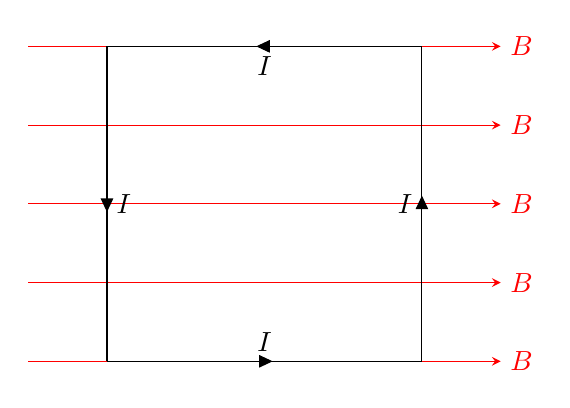
\begin{tikzpicture}
			\def\a{4};

			\begin{scope}[-stealth, red]
				\foreach \i in {0,...,\a}
				{
					\draw (-1,\i) -- (\a + 1, \i) node [right] {$B$};
				}
			\end{scope}

			\begin{scope}
				\draw (0,0) to [short, i = $I$] (\a,0);
				\draw (\a,0) to [short, i = $I$] (\a,\a);
				\draw (\a,\a) to [short, i = $I$] (0,\a);
				\draw (0,\a) to [short, i = $I$] (0,0);
			\end{scope}
		\end{tikzpicture}
	\end{figure}
	Describe the motion of the loop.
\end{question}

\begin{solution}
	The force on the right side of the square loop is directed inwards, and the force on the left side is directed outwards.
	These forces are equal in magnitude.
	\begin{align*}
		F & = I a B
	\end{align*}
	The forces on the upper and lower sides of the loop are zero, as the directions of the magnetic field and $\overrightarrow{I \dif l}$ are the same.\\
	Therefore, as the forces on the left and right sides are opposite in direction, there is no net force on the loop, but there is a net torque.\\
	Hence, the loop will rotate around an axis as shown.\\
	After the loop rotates, the upper and lower sides will have a force acting on them.
	However, due to the directions of the forces, it will have no effect on the motion of the loop.
	The forces only work towards deforming the loop.\\
	Therefore, the net torque on the loop is
	\begin{align*}
		\overrightarrow{\tau} & = 2 \left( \frac{a}{2} \cdot I a B \cdot \sin \theta \right) \hat{z} \\
                                      & = I a^2 B \sin \theta \hat{z}                                        \\
                                      & = I A B \sin \theta \hat{z}                                          \\
                                      & = I \overrightarrow{A} \times \overrightarrow{B}                     \\
                                      & = \overrightarrow{\mu} \times \overrightarrow{B}
	\end{align*}
\end{solution}

\begin{question}
	Find the force between two wires of length $l$, carrying currents $I_1$ and $I_2$, respectively, separated by a distance $r$, where $l >> r$.
\end{question}

\begin{solution}
	\begin{align*}
		F & = I_2 l B_1                     \\
                  & = I_2 l \frac{\mu_0 I}{2 \pi r} \\
                  & = \frac{\mu_0 I_1 I_2 l}{2 \pi r}
	\end{align*}
\end{solution}

\section{Ampere's Law}

\begin{law}[Ampere's Law]
	Let $C$ be a virtual closed loop.
	\begin{equation*}
		\oint\limits_{C} \overrightarrow{B} \cdot \overrightarrow{\dif l} = \mu_0 I_{\textnormal{enclosed}}
	\end{equation*}
	\label{Ampere's_Law}
\end{law}

\begin{question}
	A cylindrical wire of radius $R$ is carrying current with current density $\overrightarrow{j} = j \hat{z}$.
	Find the magnetic field at a distance $r > R$ from the centre of the wire.
\end{question}

\begin{solution}
	\begin{align*}
		\overrightarrow{B} & = B_r \hat{r} + B_{\varphi} \hat{\varphi} + B_z \hat{z}
	\end{align*}
	Due to the symmetry of the cylinder, $B$ is independent of $\varphi$.\\
	As the wire is infinite, $B$ is independent of $z$.\\
	By the \nameref{Biot-Savart_Law}, $B$ should be in the $\hat{\varphi}$ direction only.\\
	Therefore,
	\begin{align*}
		\overrightarrow{B}(r) & = B_{\varphi}(r) \hat{\varphi}
	\end{align*}
	Consider a circular virtual Ampere loop with radius $r$.\\
	Therefore, by \nameref{Ampere's_Law},
	\begin{align*}
		\oint \overrightarrow{B} \cdot \overrightarrow{\dif l} & = \mu_0 I                 \\
		\therefore B \cdot 2 \pi r                             & = \mu_0 I                 \\
		\therefore B                                           & = \frac{\mu_0 I}{2 \pi r} \\
		\therefore \overrightarrow{B}                          & = \frac{\mu_0 I}{2 \pi r} \hat{\varphi}
	\end{align*}
	If $r > R$,
	\begin{align*}
		\overrightarrow{B} & = \frac{\mu_0 j \pi R^2}{2 \pi r} \hat{\varphi} \\
                                   & = \frac{\mu_0 j R^2}{2 r} \hat{\varphi}
	\end{align*}
	If $r < R$,
	\begin{align*}
		\overrightarrow{B} & = \frac{\mu_0 j \pi r^2}{2 \pi r} \hat{\varphi} \\
                                   & = \frac{\mu_0 j r}{2} \hat{\varphi}
	\end{align*}
	Therefore,
	\begin{align*}
		\overrightarrow{B} &=
			\begin{cases}
				\frac{\mu_0 j r}{2} \hat{\varphi}     & ;\quad r < R \\
				\frac{\mu_0 j R^2}{2 r} \hat{\varphi} & ;\quad r > R \\
			\end{cases}
	\end{align*}
\end{solution}

\begin{question}
	An infinite plate in the $x$-$y$ plane is carrying current in the positive $x$ direction.
	The current density is $k = \frac{I}{l}$.
\end{question}

\begin{solution}
	Consider a square virtual Ampere loop, directed anti-clockwise, as shown.
	\begin{figure}[H]
		\begin{tikzpicture}
			\def\xMIN{-5};
			\def\xMAX{5};
			\def\yMIN{-5};
			\def\yMAX{5};

			\def\l{2};
			\def\h{3};

			\begin{scope}[stealth-stealth, lightgray]
				\draw (\xMIN,0) -- (\xMAX,0) node [right] {$y$};
				\draw (0,\yMIN) -- (0,\yMAX) node [above] {$z$};
			\end{scope}

			\begin{scope}
				\draw (-\l/2,-\h/2) rectangle (\l/2,\h/2);
			\end{scope}

			\begin{scope}
				\foreach \x in {\xMIN,...,\xMAX}
				{
					\node at (\x,0) {$\odot$};
				}
			\end{scope}
		\end{tikzpicture}
	\end{figure}
	Therefore by \nameref{Ampere's_Law},
	\begin{align*}
		\oint \overrightarrow{B} \cdot \overrightarrow{\dif l} &= \mu_0 I_{\textnormal{enclosed}}\\
		\therefore 2 |B| l &= \mu_0 k l\\
		\therefore |B| &= \frac{\mu_0 k}{2}
	\end{align*}
	Therefore,
	\begin{align*}
		\overrightarrow{B} &=
			\begin{cases}
				-\frac{\mu_0 k}{2} \hat{y} & ;\quad z > 0 \\
				\frac{\mu_0 k}{2} \hat{y}  & ;\quad z < 0 \\
			\end{cases}
	\end{align*}
\end{solution}

\section{Differential Form of Ampere's Law}

\begin{law}[Differential Form of Ampere's Law]
	\begin{align*}
		\overrightarrow{\nabla} \times \overrightarrow{B} & = \mu_0 \overrightarrow{j}
	\end{align*}
	\label{Differential_Form_of_Ampere's_Law}
\end{law}

\begin{proof}
	Consider a closed virtual loop $C$ with surface area $S$.\\
	Therefore, by \nameref{Ampere's_Law},
	\begin{align*}
		\oint\limits_{C} \overrightarrow{B} \cdot \overrightarrow{\dif l} & = \mu_0 I_{\textnormal{enclosed}}
	\end{align*}
	The loop can be considered to be made up of two virtual loops as shown.
	\begin{figure}[H]
		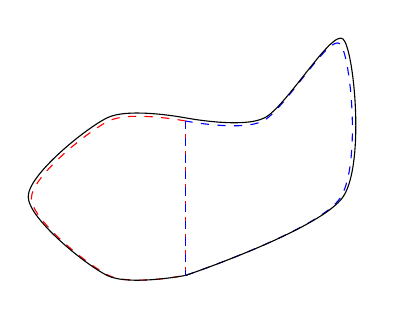
\begin{tikzpicture}
			\begin{scope}[red, scale = 0.98, dashed]
				\draw plot [smooth, tension = 0.5] coordinates { (0,2) (-1,2) (-2,1) (-1,0) (0,0) };
				\draw (0,0) -- (0,2);
			\end{scope}
			\begin{scope}[blue, scale = 0.98, dashed]
				\draw plot [smooth, tension = 0.5] coordinates { (0,0) (2,1) (2,3) (1,2) (0,2) };
				\draw (0,2) -- (0,0);
			\end{scope}
			\draw plot [smooth, tension = 0.5] coordinates { (0,2) (-1,2) (-2,1) (-1,0) (0,0) };
			\draw plot [smooth, tension = 0.5] coordinates { (0,0) (2,1) (2,3) (1,2) (0,2) };
		\end{tikzpicture}
	\end{figure}
	Similarly, let the area enclosed by the loop be divided into small virtual loops $C_i$ of area $a_i$.\\
	\begin{figure}[H]
		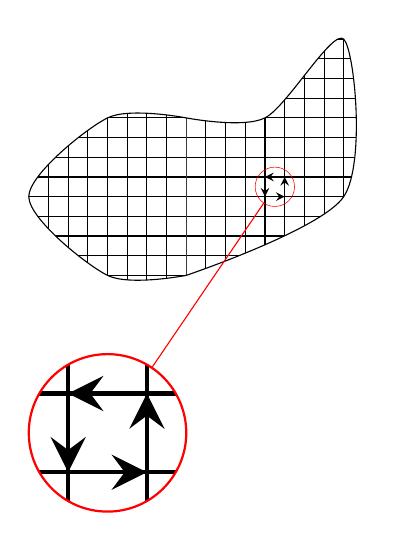
\begin{tikzpicture}
			[spy using outlines={circle, magnification=4, size=2cm, connect spies}]
			\begin{scope}
				\clip plot [smooth, tension = 0.5] coordinates { (0,2) (-1,2) (-2,1) (-1,0) (0,0) };
	
				\draw[step = 0.25] (-5,-5) grid (5,5);
			\end{scope}
			\begin{scope}
				\clip plot [smooth, tension = 0.5] coordinates { (0,0) (2,1) (2,3) (1,2) (0,2) };
	
				\draw[step = 0.25] (-5,-5) grid (5,5);
			\end{scope}
			\draw plot [smooth, tension = 0.5] coordinates { (0,2) (-1,2) (-2,1) (-1,0) (0,0) };
			\draw plot [smooth, tension = 0.5] coordinates { (0,0) (2,1) (2,3) (1,2) (0,2) };
			\begin{scope}[-stealth]
				\draw (1,1) -- (1.25,1);
				\draw (1.25,1) -- (1.25,1.25);
				\draw (1.25,1.25) -- (1,1.25);
				\draw (1,1.25) -- (1,1);
			\end{scope}
			\begin{scope}
				\spy [red, size = 2cm] on (1.125,1.125) in node [right] at (-2,-2);
			\end{scope}
		\end{tikzpicture}
	\end{figure}
	Therefore,
	\begin{align*}
		\oint\limits_{C} \overrightarrow{B} \cdot \overrightarrow{\dif l} & = \sum\limits_{i} \oint\limits_{C_i} \overrightarrow{B} \cdot \overrightarrow{\dif l}
	\end{align*}
	The curl is defined as
	\begin{align*}
		(\curl B) \hat{n} & = \lim\limits_{a_i \to 0} \frac{\oint\limits_{C_i} \overrightarrow{B} \cdot \overrightarrow{\dif l}}{a_i}
	\end{align*}
	where $\hat{n}$ is perpendicular to the area $a_i$.\\
	Therefore,
	\begin{align*}
		\oint\limits_{C} \overrightarrow{B} \cdot \overrightarrow{\dif l}            & = \lim\limits_{\max a_i \to 0} \sum\limits_{i} \oint\limits_{C_i} \overrightarrow{B} \cdot \overrightarrow{\dif l} \\
                                                                                             & = \lim\limits_{\max a_i \to 0} \sum\limits_{i} (\curl B) \hat{n} a_i                                               \\
                                                                                             & = \lim\limits_{\max a_i \to 0} \sum\limits_{i} (\curl B) \overrightarrow{a_i}                                      \\
                                                                                             & = \iint\limits_{S} \curl B \cdot \overrightarrow{\dif a}                                                           \\
		\therefore \oint\limits_{C} \overrightarrow{B} \cdot \overrightarrow{\dif l} & = \iint\limits_{S} \curl B \cdot \overrightarrow{\dif a}
	\end{align*}
	~\\
	Consider a loop in the $x$-$y$ plane as shown.
	\begin{figure}[H]
		\begin{tikzpicture}
			\def\xMIN{-1};
			\def\xMAX{5};
			\def\yMIN{-1};
			\def\yMAX{5};
	
			\def\x{2};
			\def\dx{2};
			\def\y{2};
			\def\dy{2};
	
			\begin{scope}[stealth-stealth, lightgray]
				\draw (\xMIN,0) -- (\xMAX,0) node [right] {$x$};
				\draw (0,\yMIN) -- (0,\yMAX) node [above] {$y$};
			\end{scope}
	
			\begin{scope}[-stealth]
				\draw ({\x - \dx/2},{\y - \dy/2}) -- ({\x + \dx/2},{\y - \dy/2});
				\draw ({\x + \dx/2},{\y - \dy/2}) -- ({\x + \dx/2},{\y + \dy/2});
				\draw ({\x + \dx/2},{\y + \dy/2}) -- ({\x - \dx/2},{\y + \dy/2});
				\draw ({\x - \dx/2},{\y + \dy/2}) -- ({\x - \dx/2},{\y - \dy/2});
			\end{scope}
	
			\begin{scope}[dashed]
				\draw ({\x - \dx/2},{\y - \dy/2}) -- ({\x - \dx/2},0) node [below] {$x_0 - \frac{\dif x}{2}$};
				\draw ({\x + \dx/2},{\y - \dy/2}) -- ({\x + \dx/2},0) node [below] {$x_0 + \frac{\dif x}{2}$};
	
				\draw ({\x - \dx/2},{\y - \dy/2}) -- (0,{\y - \dy/2}) node [left] {$y_0 - \frac{\dif y}{2}$};
				\draw ({\x - \dx/2},{\y + \dy/2}) -- (0,{\y + \dy/2}) node [left] {$y_0 + \frac{\dif y}{2}$};
			\end{scope}
		\end{tikzpicture}
	\end{figure}
	\begin{align*}
		(\curl B) \hat{z} & = \frac{\oint\limits_{C} \overrightarrow{B} \cdot \overrightarrow{\dif l}}{\dif x \dif y}                                                                                                                                                  \\
                                  & = \quad \frac{B_x\left( x_0 , y_0 - \frac{\dif y}{2} , z_0 \right) \dif x - B_x\left( x_0 , y_0 + \frac{\dif y}{2} , z_0 \right) \dif x}{\dif x \dif y}                                                                                    \\
                                  & \quad + \frac{B_y\left( x_0 - \frac{\dif x}{2} , y_0 , z_0 \right) \dif y - B_y\left( x_0 + \frac{\dif x}{2}, y_0 , z_0 \right) \dif y}{\dif x \dif y}                                                                                     \\
                                  & = \quad \frac{\frac{B_x\left( x_0 , y_0 - \frac{\dif y}{2} , z_0 \right) \dif x \dif y - B_x\left( x_0 , y_0 + \frac{\dif y}{2} , z_0 \right) \dif x \dif y}{\dif y}}{\dif x \dif y}                                                       \\
                                  & \quad + \frac{\frac{B_y\left( x_0 - \frac{\dif x}{2} , y_0 , z_0 \right) \dif x \dif y - B_y\left( x_0 + \frac{\dif x}{2}, y_0 , z_0 \right) \dif x \dif y}{\dif x}}{\dif x \dif y}                                                        \\
                                  & = \frac{\left. -\pd{B_x}{y} \right|_{\left( x_0 , y_0 - \frac{\dif y}{2} , x_0 \right)} \dif x \dif y}{\dif x \dif y} + \frac{\left. \pd{B_y}{x} \right|_{\left( x_0 - \frac{\dif x}{2} , y_0 , x_0 \right)} \dif x \dif y}{\dif x \dif y} \\
                                  & = \left. \left( \pd{B_y}{x} - \pd{B_x}{y} \right) \right|_{(x_0, y_0, z_0)}
	\end{align*}
	Similarly for loops in the $y$-$z$ and $z$-$x$ planes.\\
	Therefore,
	\begin{align*}
		\curl B &=
			\begin{vmatrix}
				\hat{x}  & \hat{y}  & \hat{z}  \\
				\pd{}{x} & \pd{}{y} & \pd{}{z} \\
				B_x      & B_y      & B_z      \\
			\end{vmatrix}\\
			&= \overrightarrow{\nabla} \times \overrightarrow{B}
	\end{align*}
	Therefore,
	\begin{align*}
		\overrightarrow{\nabla} \times \overrightarrow{B} &= \mu_0 \overrightarrow{j}
	\end{align*}
\end{proof}

\section{Faraday's Law}

\begin{question}
	A rod of length $l$ is moving with velocity $v$ in a region of uniform magnetic field $B$ as shown.
	\begin{figure}[H]
		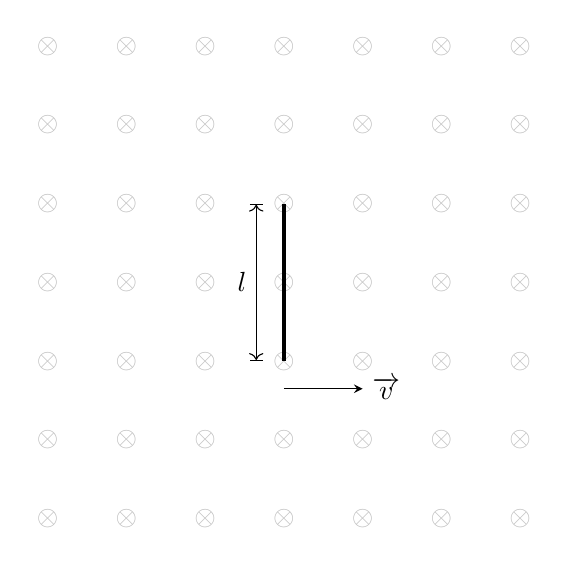
\begin{tikzpicture}
			\def\l{2};
			\def\F{1};

			\begin{scope}[lightgray]
				\foreach \x in {-3,...,3}
				{
					\foreach \y in {-3,...,3}
					{
						\node at (\x,\y) {$\otimes$};
					}
				}
			\end{scope}

			\draw[ultra thick] (0,-\l/2) -- (0,\l/2);

			\draw[-stealth, yshift = -10] (0,-\l/2) -- ++(0:\F) node [right] {$\overrightarrow{v}$};

			\draw[xshift = -10, |<->|] (0,-\l/2) -- (0,\l/2) node [midway, left] {$l$};
		\end{tikzpicture}
	\end{figure}
	Find the potential difference $V$ generated between its ends.
\end{question}

\begin{solution}
	As the rod is moving under a magnetic field, there will be a force acting on every charged particle in the rod.
	The force on positively charged particles is upwards and the force on negatively charged particles if downwards.\\
	Therefore, there will be a charge distribution created inside the rod.
	Therefore, there will be an electric field between the ends of the rod.
	Hence, there will also be a potential difference generated between its ends.\\
	Consider a charged particle of charge $q$ in the rod.\\
	The force required for it to move to the end of the rod is equal to the force acting on it due to its movement under the magnetic field.\\
	Therefore,
	\begin{align*}
		q E            & = q v B \\
		\therefore E l & = B v l \\
		\therefore V   & = B v l
	\end{align*}
\end{solution}

\begin{definition}[Electromotive Force]
	\begin{equation*}
		\varepsilon = \oint \left( \overrightarrow{E} + \overrightarrow{v} \times \overrightarrow{B} \right) \cdot \overrightarrow{\dif l}
	\end{equation*}
\end{definition}

Consider a rectangular loop of height $L$ moving with velocity $v$ as shown.
\begin{figure}[H]
	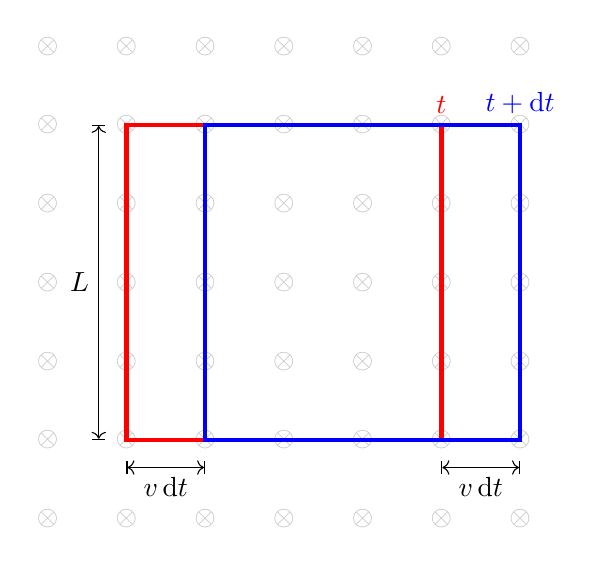
\begin{tikzpicture}
		\def\L{4};
		\def\vdt{1cm};
		\begin{scope}[lightgray]
			\foreach \x in {-3,...,3}
			{
				\foreach \y in {-3,...,3}
				{
					\node at (\x,\y) {$\otimes$};
				}
			}
		\end{scope}
		\begin{scope}[red, ultra thick]
			\draw (-\L/2,-\L/2) rectangle (\L/2,\L/2) node [above] {$t$};
		\end{scope}
		\begin{scope}[blue, ultra thick, xshift = \vdt]
			\draw (-\L/2,-\L/2) rectangle (\L/2,\L/2) node [above] {$t + \dif t$};
		\end{scope}
		\begin{scope}
			\draw[xshift = -10, |<->|] (-\L/2,-\L/2) -- (-\L/2,\L/2) node [midway, left] {$L$};
		\end{scope}
		\begin{scope}[yshift = -10, |<->|]
			\draw (-\L/2,-\L/2) -- ++(0:\vdt) node [midway, below] {$v \dif t$};
			\draw (\L/2,-\L/2) -- ++(0:\vdt) node [midway, below] {$v \dif t$};
		\end{scope}
	\end{tikzpicture}
\end{figure}
\begin{align*}
	\varepsilon & = \oint \left( \overrightarrow{E} + \overrightarrow{v} \times \overrightarrow{B} \right) \cdot \overrightarrow{\dif l}                                     \\
                    & = \oint \overrightarrow{E} \cdot \overrightarrow{\dif l} + \oint \left( \overrightarrow{v} \times \overrightarrow{B} \right) \cdot \overrightarrow{\dif l} \\
                    & = 0 + B L v
\end{align*}
\begin{align*}
	\dif \Phi_B & = \Phi_B(t + \dif t) - \Phi_B(t)                                                                                                  \\
                    & = \quad \left( \text{flux due to common area} + B_2 L v \dif t \right)\\
		    &\quad - \left( \text{flux due to common area} + B_1 L v \dif t \right) \\
                    & = (B_2 L v - B_1 L v) \dif t
\end{align*}
Therefore,
\begin{align*}
	B_2 L v - B_1 L v      & = \dod{\Phi_B}{t} \\
	\therefore \varepsilon & = -\dod{\Phi_B}{t}
\end{align*}
In general,
\begin{law}[Faraday's Law]
	For a loop of area $S$,
	\begin{align*}
		\oint\limits_{\partial S} \left( \overrightarrow{E} + \overrightarrow{v} \times \overrightarrow{B} \right) \cdot \overrightarrow{\dif l} & = -\dod{}{t} \iint\limits_{S} \overrightarrow{B} \cdot \overrightarrow{\dif a}
	\end{align*}
	If the loop is not moving,
	\begin{align*}
		\oint\limits_{\partial S} \overrightarrow{E} \cdot \overrightarrow{\dif l} & = -\dod{}{t} \iint\limits_{S} \overrightarrow{B} \cdot \overrightarrow{\dif a}
	\end{align*}
	By Stoke's Theorem,
	\begin{align*}
		\iint\limits_{S} \left( \overrightarrow{\nabla} \times \overrightarrow{E} \right) \cdot \overrightarrow{\dif a} & = \iint\limits_{S} -\dpd{\overrightarrow{B}}{t} \cdot \overrightarrow{\dif a} \\
		\therefore \overrightarrow{\nabla} \times \overrightarrow{E}                                                    & = -\dpd{\overrightarrow{B}}{t}
	\end{align*}
	\label{Faraday's_Law}
\end{law}

\begin{law}[Lenz's Law]
	The direction of an induced current is in a direction such that it opposes the change in the magnetic flux responsible for its creation.
	\label{Lenz's_Law}
\end{law}

\begin{question}
	A solenoid of infinite length has $n$ turns per unit length.
	The current through it is
	\begin{align*}
		I &= \alpha t
	\end{align*}
	Find the induced electric field, at a point inside it.
\end{question}

\begin{solution}
	\begin{figure}[H]
		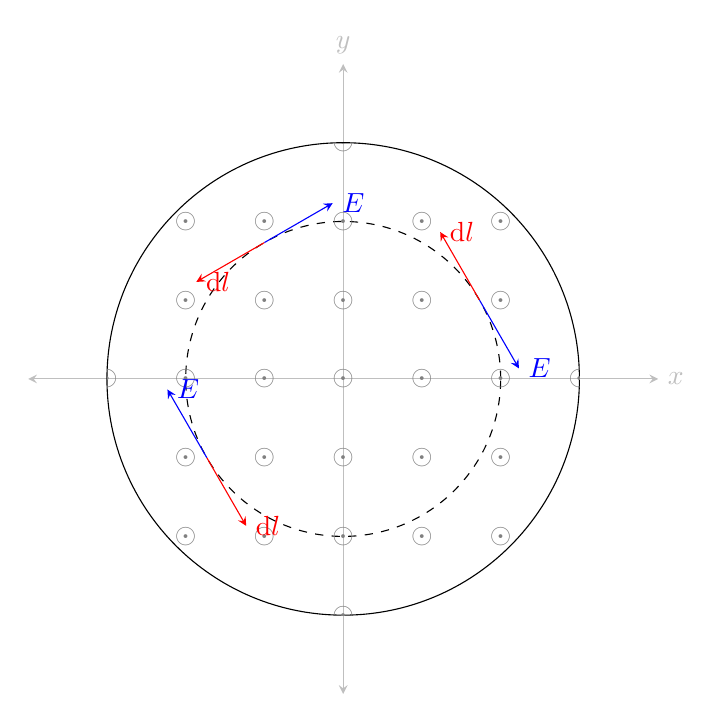
\begin{tikzpicture}
			\def\xMIN{-4};
			\def\xMAX{4};
			\def\yMIN{-4};
			\def\yMAX{4};

			\def\R{3};
			\def\r{2};
			\def\angle{30};
			\def\F{1};

			\begin{scope}[stealth-stealth, lightgray]
				\draw (\xMIN,0) -- (\xMAX,0) node [right] {$x$};
				\draw (0,\yMIN) -- (0,\yMAX) node [above] {$y$};
			\end{scope}

			\begin{scope}[-stealth]
				\draw (0,0) circle (\R);
			\end{scope}

			\begin{scope}[dashed]
				\draw (0,0) circle (\r);
			\end{scope}

			\begin{scope}[gray]
				\clip (0,0) circle (\R);

				\foreach \x in {\xMIN,...,\xMAX}
				{
					\foreach \y in {\yMIN,...,\yMAX}
					{
						\node at (\x,\y) {$\odot$};
					}
				}
			\end{scope}

			\begin{scope}[-stealth]
				\foreach \ang in {30,120,210}
				{
					\draw[red] (\ang:\r) -- ++(\ang + 90 : \F) node [right] {$\dif l$};
					\draw[blue] (\ang:\r) -- ++(\ang - 90 : \F) node [right] {$E$};
				}
			\end{scope}
		\end{tikzpicture}
	\end{figure}
	Consider a virtual loop of radius $r$, directed anti-clockwise.\\
	Therefore, by \nameref{Faraday's_Law},
	\begin{align*}
		\oint \overrightarrow{E} \cdot \overrightarrow{\dif l} &= -\dod{}{t}\left( B \cdot \pi r^2 \right)\\
		&= -\dod{}{t}\left( \mu_0 \alpha t n \cdot \pi r^2 \right)\\
		&= -\mu_0 \alpha n \pi r^2\\
		\therefore E \cdot 2 \pi r &= -\mu_0 \alpha n \pi r^2\\
		\therefore E &= -\frac{\mu_0 \alpha n r}{2}
	\end{align*}
	Therefore, as $E$ is negative, it is opposite to the direction of the loop.\\
	Therefore,
	\begin{align*}
		E &= -\frac{\mu_0 \alpha n r}{2} \hat{\varphi}
	\end{align*}
\end{solution}

\section{Inductors}

Consider a solenoid with $n$ turns per unit length.\\
Therefore,
\begin{align*}
	B &= \mu_0 I n
\end{align*}
and
\begin{align*}
	\varepsilon &= -\dod{\Phi_B}{t}\\
\end{align*}
Therefore,
\begin{align*}
	\varepsilon &\propto \dod{I}{t}
\end{align*}

\begin{definition}[Self inductance]
	\begin{align*}
		L &= \frac{\varepsilon}{\dod{I}{t}}
	\end{align*}
	is called self inductance.
\end{definition}

\begin{question}
	Find the self inductance of a solenoid with length $l$, and $N$ turns of radius $R$.
\end{question}

\begin{solution}
	Let the number of turns per unit length be
	\begin{align*}
		n &= \frac{N}{l}
	\end{align*}
	Let $\varepsilon_1$ be the voltage across each loop of the solenoid.\\
	Therefore,
	\begin{align*}
		\varepsilon_1 &= -\dot{\varphi_B}
	\end{align*}
	Therefore, the voltage between the ends of the solenoid is,
	\begin{align*}
		\varepsilon_L &= N \varepsilon_1\\
		\therefore L \dot{I} &= N \dot{\varphi_B}\\
		&= N \dod{}{t}\left( \mu_0 I n \pi R^2 \right)\\
		&= N \mu_0 \dot{I} n \pi R^2\\
		&= \mu_0 \frac{N^2}{l} \pi R^2 \dot{I}\\
		\therefore L &= \mu_0 \frac{N^2}{l} \pi R^2\\
		&= \mu_0 n^2 l A
	\end{align*}
\end{solution}

\subsection{Energy Stored in an Inductor}

Consider an inductor of length $l$, cross-sectional area $A$, and inductance $L$.
\begin{align*}
	P &= \varepsilon_L I\\
	\therefore \dod{U_L}{t} &= L \dot{I} I\\
	\therefore U_L &= \frac{1}{2} L I^2
\end{align*}

\subsection{Energy Density}

Consider an inductor of length $l$, cross-sectional area $A$, and inductance $L$.
\begin{align*}
	U_L &= \frac{1}{2} L I^2\\
	&= \frac{1}{2} \mu_0 n^2 l A \frac{B^2}{{\mu_0}^2 n^2}\\
	&= \frac{B^2}{2 \mu_0} l A
\end{align*}
Therefore,
\begin{align*}
	u_L &= \frac{U_L}{V}\\
	&= \frac{B^2}{2 \mu_0}\\
	&= \frac{1}{2} \frac{1}{\mu_0} B^2
\end{align*}

\section{LR Series Circuit}

\begin{figure}[H]
	\begin{circuitikz}
		\draw 
			(0,0) to [short, i = $I(t)$] (0,2)
			(0,2) to [R = $R$] (3,2)
			(3,2) to [L = $L$] (3,0)
			(3,0) to [battery1 = $\varepsilon$] (0,0);
	\end{circuitikz}
\end{figure}

\subsection{Current in the Inductor}

\begin{align*}
	\oint \overrightarrow{E} \cdot \overrightarrow{\dif l} &= 0\\
	\therefore -\varepsilon + I R + L \dot{I} &= 0\\
	\therefore \dot{I} + \frac{R}{L} I &= \frac{\varepsilon}{L}\\
	\therefore \dod{I}{t} + \frac{R}{L} I &= \frac{\varepsilon}{L}\\
	\therefore I &= \frac{1}{e^{\int \frac{R}{L} \dif t}} \int e^{\frac{R}{L} \dif t} \frac{\varepsilon}{L} \dif t\\
	&= \frac{\varepsilon}{R} \left( 1 - e^{-\frac{R}{L} t} \right)
\end{align*}

\begin{definition}[Time constant of LR circuit]
	$\tau = \frac{L}{R}$ is called the time constant of a circuit with a resistor of resistance $R$ and a inductor of inductance $L$ connected in series.
\end{definition}

\subsection{Mutual Inductance}

\begin{definition}[Mutual Inductance]
	Consider two loops, loop $1$ and loop $2$.\\
	Let there be a current $I_1$ in loop $1$.\\
	Therefore, a magnetic field $B_1$ will be induced.\\
	Therefore, there will be a magnetic flux, ${\Phi_{B}}_{2 1}$, due to $B_1$, in loop $2$.\\
	As a result, there will be a potential difference, $\varepsilon_2$, induced in loop $2$.
	Hence, there will be a current, $I_2$, induced in loop $2$.\\
	The mutual inductance of the two loops is defined as
	\begin{align*}
		\varepsilon_2 &= -M_{2 1} \dot{I_1}
	\end{align*}
	\begin{equation*}
		M_{1 2} = M_{2 1} = M
	\end{equation*}
\end{definition}

\begin{theorem}
	Consider two loops, loop $1$ and loop $2$.\\
	Then,
	\begin{equation*}
		M_{1 2} = M_{2 1} = M
	\end{equation*}
\end{theorem}

\begin{question}
	Find the mutual inductance of two concentric rings of radii $r_1 << r_2$.
\end{question}

\begin{solution}
	Let there be a current $I_2$ in the ring of radius $r_2$.\\
	Therefore, the magnetic field at the centre, due to $I_2$ is,
	\begin{align*}
		B_2 &= \frac{\mu_0 I_2}{2 r_2}\\
		\therefore {\Phi_B}_{1 2} &= \frac{\mu_0 I_2}{2 r_2} \cdot \pi {r_1}^2\\
		\therefore \varepsilon_1 &= -\dot{{\Phi_B}_{1 2}}\\
		&= -\frac{\mu_0 \pi {r_1}^2}{2 r_2} \dot{I_2}\\
		\therefore \frac{\varepsilon_i}{\dot{I_2}} &= \frac{\mu_0 \pi {r_1}^2}{2 r_2}\\
		\therefore M &= \frac{\mu_0 \pi {r_1}^2}{2 r_2}
	\end{align*}
\end{solution}

\section{Transformers}

Two coils of equal radii have $n_1$ and $n_2$ turns respectively.
They are connected as shown.
\begin{figure}[H]
	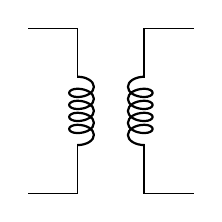
\begin{tikzpicture}
		\draw node [transformer] at (0,0) {};
	\end{tikzpicture}
\end{figure}
Coil $1$ is connected to a variable voltage $\varepsilon_1$.
Therefore, there is an induced magnetic field $B$ acting on both coils.\\
Therefore, there is an induced magnetic flux through both coils.\\
Hence, there will be an induced emf, $\varepsilon_2$ across the second coil.
\begin{align*}
	\varepsilon_1 & = -n_1 \dot{\varphi_B} \\
	\varepsilon_2 & = -n_2 \dot{\varphi_B}
\end{align*}
Therefore, as the cross-sectional area of the coils is equal, the flux through them is equal.\\
Therefore,
\begin{align*}
	\frac{\varepsilon_1}{n_1} & = \frac{\varepsilon_2}{n_2} \\
	\therefore \varepsilon_2  & = \varepsilon_1 \frac{n_2}{n_1}
\end{align*}

\section{Maxwell's Correction to Ampere's Law}
By \nameref{Ampere's_Law},
\begin{align*}
	\overrightarrow{\nabla} \times \overrightarrow{B} & = \mu_0 \cdot \overrightarrow{j}
\end{align*}
Therefore, taking the divergence of both sides,
\begin{align*}
	\overrightarrow{\nabla} \cdot \overrightarrow{\nabla} \times \overrightarrow{B} & = 0              \\
	\intertext{but}
	\overrightarrow{\nabla} \cdot \left( \mu_0 \overrightarrow{j} \right)           & = -\dpd{\rho}{t} \\
                                                                                        & \neq 0
\end{align*}
Therefore, there must be a missing term in the RHS.\\
Therefore,
\begin{align*}
	\overrightarrow{\nabla} \times \overrightarrow{B}                                          & = \mu_0 \overrightarrow{j} + \overrightarrow{g}                                                             \\
	\therefore \overrightarrow{\nabla} \cdot \overrightarrow{\nabla} \times \overrightarrow{B} & = \mu_0 \overrightarrow{\nabla} \cdot \overrightarrow{j} + \overrightarrow{\nabla} \cdot \overrightarrow{g} \\
	\therefore 0                                                                               & = -\dpd{\rho}{t} + \overrightarrow{\nabla} \cdot \overrightarrow{g}                                         \\
	\therefore \overrightarrow{\nabla} \cdot \overrightarrow{g}                                & = \mu_0 \dpd{\rho}{t}
\end{align*}
By \nameref{Differential_Form_of_Gauss'_Law},
\begin{align*}
	\overrightarrow{\nabla} \cdot \overrightarrow{E}                                                  & = \frac{\rho}{\varepsilon_0} \\
	\therefore \overrightarrow{\nabla} \cdot \left( \varepsilon_0 \overrightarrow{E} \right)          & = \rho                       \\
	\therefore \overrightarrow{\nabla} \cdot \left( \varepsilon_0 \dpd{\overrightarrow{E}}{t} \right) & = \dpd{\rho}{t}
\end{align*}
Therefore,
\begin{align*}
	\overrightarrow{\nabla} \cdot \overrightarrow{g} & = \mu_0 \dpd{\rho}{t}                                   \\
                                                         & = \overrightarrow{\nabla} \cdot \overrightarrow{g}      \\
                                                         & = \mu_0 \varepsilon_0 \cdot \dpd{\overrightarrow{E}}{t} \\
	\therefore g                                     & = \mu_0 \varepsilon_0 \dpd{\overrightarrow{E}}{t}
\end{align*}

\begin{definition}[Displacement current density]
	\begin{align*}
		\overrightarrow{j_D} & = \varepsilon_0 \dpd{\overrightarrow{E}}{t}
	\end{align*}
	is called the displacement current density.
\end{definition}

Therefore,
\begin{law}[Maxwell's Correction to Ampere's Law]
	\begin{align*}
		\overrightarrow{\nabla} \times \overrightarrow{B} & = \mu_0 \overrightarrow{j} + \mu_0 \varepsilon_0 \dpd{\overrightarrow{E}}{t} \\
                                                                  & = \mu_0 \overrightarrow{j} + \mu_0 \overrightarrow{j_D}
	\end{align*}
	Therefore,
	\begin{align*}
		\oint\limits_{\partial S} \overrightarrow{B} \cdot \overrightarrow{\dif l} & = \mu_0 \iint\limits_{S} \overrightarrow{j} \cdot \overrightarrow{\dif A} + \mu_0 \varepsilon_0 \dod{}{t}\iint\limits_{S} \overrightarrow{E} \cdot \overrightarrow{\dif A} \\
                                                                                           & = \mu_0 I \cdot \overrightarrow{\dif A} + \mu_0 I_D
	\end{align*}
	\label{Maxwell's_Correction_to_Ampere's_Law}
\end{law}

\begin{landscape}

\doublespacing

\section{Maxwell's Equations}

\begin{tabular}{|l||l|l|}
	\hline
	Law                        & Integral Form                                                                                                                                                                                                                               & Differential Form                                                                                                                \\ [1.5ex]
	\hline
	Gauss' Law for Electricity & $\displaystyle \oiint\limits_{\partial V} = \dfrac{1}{\varepsilon_0} \iiint\limits_{V} \rho \dif^3 r$                                                                                                                                       & $\overrightarrow{\nabla} \cdot \overrightarrow{E} = \dfrac{\rho}{\varepsilon_0}$                                                 \\ [1.5ex]

	Gauss' Law for Magnetism   & $\displaystyle \oint\limits_{\partial S} \overrightarrow{E} \cdot \overrightarrow{\dif l} = -\dod{}{t} \iint\limits_{S} \overrightarrow{B} \cdot \dif \overrightarrow{A}$                                                                   & $\overrightarrow{\nabla} \times \overrightarrow{E} = -\dpd{\overrightarrow{B}}{t}$                                               \\ [1.5ex]

	Faraday's Law              & $\displaystyle \oiint\limits_{S} \overrightarrow{B} \cdot \dif \overrightarrow{A} = 0$                                                                                                                                                      & $\overrightarrow{\nabla} \cdot \overrightarrow{B} = 0$                                                                           \\ [1.5ex]

	Ampere's Law               & $\displaystyle \overrightarrow{B} \cdot \overrightarrow{\dif l} = \mu_0 \iint\limits_{S} \overrightarrow{j} \cdot \dif \overrightarrow{A} + \mu_0 \varepsilon_0 \dod{}{t}\iint\limits_{S} \overrightarrow{E} \cdot \dif \overrightarrow{A}$ & $\overrightarrow{\nabla} \times \overrightarrow{B} = \mu_0 \overrightarrow{j} + \mu_0 \varepsilon_0 \dpd{\overrightarrow{E}}{t}$ \\ [1.5ex]

	\hline
\end{tabular}

\end{landscape}

\singlespacing

\begin{question}
	A capacitor has circular plates of radius $a$ with distance $d$ between them.\\
	It is connected by wires with distance $L$ between the wires.\\
	A rod is kept connecting the wires, as shown.\\
	A constant magnetic field $B$ is directed inwards as shown.
	\begin{figure}[H]
		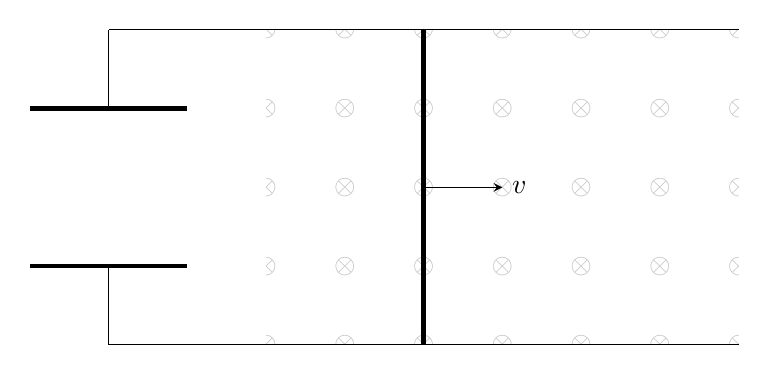
\begin{tikzpicture}
			\def\a{1};
			\def\d{2};
			\def\L{4};
			\def\F{1};
			
			\coordinate (bottom plate centre) at (0,-\d/2);
			\coordinate (top plate centre) at (0,\d/2);
			
			\begin{scope}[lightgray]
				\clip (\L/2,-\L/2) rectangle (2*\L,\L/2);
				\foreach \x in {0,...,10}
				{
					\foreach \y in {-10,...,10}
					{
						\node at (\x,\y) {$\otimes$};
					}
				}
			\end{scope}

			\begin{scope}[ultra thick]
				\draw ($ (bottom plate centre) + (-\a,0) $) -- ($ (bottom plate centre) + (\a,0) $);
				\draw ($ (top plate centre) + (-\a,0) $) -- ($ (top plate centre) + (\a,0) $);
			\end{scope}

			\begin{scope}
				\draw (bottom plate centre) -- (0,-\L/2);
				\draw (top plate centre) -- (0,\L/2);

				\draw (0,-\L/2) -- (2*\L,-\L/2);
				\draw (0,\L/2) -- (2*\L,\L/2);
			\end{scope}

			\begin{scope}[ultra thick]
				\draw (\L,\L/2) -- (\L,-\L/2);
			\end{scope}

			\begin{scope}
				\draw [-stealth] (\L,0) -- ++(\F,0) node [right] {$v$};
			\end{scope}
		\end{tikzpicture}
	\end{figure}
	The rod is moving to the right with $v = \alpha t^2$.\\
	Find the magnetic field induced between the plates of the capacitor.
\end{question}

\begin{solution}
	As the rod is moving, there is an induced emf $\varepsilon$ between the ends of the rod.\\
	Therefore, the system is equivalent to
	\begin{figure}[H]
		\begin{circuitikz}
			\draw (0,0) to [C = $C$] (0,4);
			\draw (0,4) to (4,4);
			\draw (4,0) to [battery1 = $\varepsilon$] (4,4);
			\draw (4,0) to (0,0);
		\end{circuitikz}
	\end{figure}
	Therefore,
	\begin{align*}
		C           & = \frac{A \varepsilon_0}{d}       \\
                            & = \varepsilon_0 \frac{\pi a^2}{d} \\
		\varepsilon & = v B L                           \\
                            & = \alpha t^2 B L
	\end{align*}
	Let the charge on the plates of the capacitor by $+Q$ and $-Q$.\\
	Therefore,
	\begin{align*}
		Q & = C \varepsilon \\
                  & = \varepsilon_0 \frac{\pi a^2}{d} \alpha t^2 B L
	\end{align*}
	The electric field between the capacitor plates is
	\begin{align*}
		E & = \frac{\varepsilon}{d} \\
                  & = \frac{\alpha t^2 B L}{d}
	\end{align*}
	Consider a virtual Ampereian loop of radius $r$, between the capacitor plates.\\
	Let this loop be directed clockwise if seen from above.\\
	Let the magnetic field acting on the loop be $\tilde{B}$.\\
	Therefore, by \nameref{Maxwell's_Correction_to_Ampere's_Law},
	\begin{align*}
		\oint \overrightarrow{B} \cdot \overrightarrow{\dif l} & = \cancelto{0}{\mu_0 \iint \overrightarrow{j} \cdot \dif \overrightarrow{A}} + \mu_0 \varepsilon_0 \dod{}{t}\iint \overrightarrow{E} \cdot \dif \overrightarrow{A} \\
                                                                       & = \mu_0 \varepsilon_0 \dod{}{t}\left( \frac{\alpha t^2 B L}{d} \pi r^2 \right)                                                                                     \\
		\therefore \tilde{B} \cdot 2 \pi r                     & = \mu_0 \varepsilon_0 \frac{2 \alpha t B L}{d} \pi r^2                                                                                                             \\
		\therefore \tilde{B}                                   & = \frac{\mu_0 \varepsilon_0 \alpha B L}{d} t r
	\end{align*}
	Therefore, as $\overrightarrow{\tilde{B}}$ is positive, it is directed parallel to $\dif l$.\\
	Therefore, it supports its cause.\\
	In general, the magnetic field induced due to a change in $\Phi_B$ opposes its own cause, and the magnetic field induced due to a change in $\Phi_E$ supports it own cause.
\end{solution}

\begin{question}
	A capacitor with circular plates of radius $a$ and distance $d$ between them is connected to a battery of voltage $V$.\\
	The capacitor is filled with a liquid dielectric of dielectric constant $\kappa$.\\
	The dielectric is leaking through the bottom, such that the level of the liquid is falling with velocity $u$.\\
	Find the magnetic field inside the capacitor and the displacement current.
	\begin{figure}[H]
		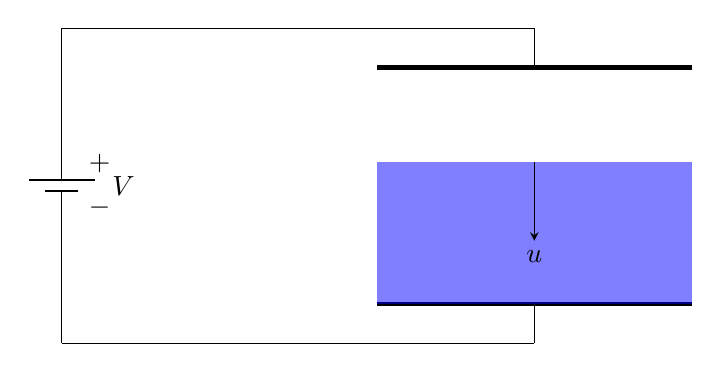
\begin{tikzpicture}
			\def\a{2};
			\def\d{3};
			\def\L{4};
			\def\F{1};
			\def\h{0.6*\d};

			\coordinate (bottom plate centre) at (3*\a,-\d/2);
			\coordinate (top plate centre) at (3*\a,\d/2);

			\begin{scope}[ultra thick]
				\draw ($ (bottom plate centre) + (-\a,0) $) -- ($ (bottom plate centre) + (\a,0) $);
				\draw ($ (top plate centre) + (-\a,0) $) -- ($ (top plate centre) + (\a,0) $);
			\end{scope}

			\begin{scope}
				\draw (bottom plate centre) -- (3*\a,-\L/2);
				\draw (top plate centre) -- (3*\a,\L/2);

				\draw (0,-\L/2) -- (3*\a,-\L/2);
				\draw (0,\L/2) -- (3*\a,\L/2);

				\draw (0,\L/2) to [battery1 = $V$] (0,-\L/2);
			\end{scope}
			\begin{scope}
				\fill [blue, opacity = 0.5] ($ (bottom plate centre) + (-\a,0) $) rectangle ($ (bottom plate centre) + (\a,\h) $);
				\draw [-stealth] ($ (bottom plate centre) + (0,\h) $) -- ++(-90:\F) node [below] {$u$};
			\end{scope}
		\end{tikzpicture}
	\end{figure}
\end{question}

\begin{solution}
	The capacitor is equivalent to a capacitor filled completely with the dielectric connected in series with a capacitor with a vacuum inside it.\\
	Therefore,
	\begin{align*}
		\frac{1}{C} & = \frac{1}{\varepsilon_0 \frac{A}{u t}} + \frac{1}{\varepsilon_0 \kappa \frac{A}{d - u t}}            \\
                            & = \frac{1}{\varepsilon_0 A} \left( \frac{1}{\frac{1}{u t}} + \frac{1}{\frac{\kappa}{d - u t}} \right) \\
                            & = \frac{1}{\varepsilon_0 A} \left( u t + \frac{d - u t}{\kappa} \right)                               \\
                            & = \frac{1}{\varepsilon_0 A} \left( \frac{d}{k} + u t \left( 1 - \frac{1}{k} \right) \right)
	\end{align*}
	Therefore,
	\begin{align*}
		C & = \varepsilon_0 \frac{A}{\frac{d}{k} + u t \left( \frac{k - 1}{k} \right)} \\
                  & = \varepsilon_0 \kappa \frac{A}{d + u t (\kappa - 1)}
	\end{align*}
	Therefore, the charge on the bottom plate of the capacitor is,
	\begin{align*}
		Q & = C V \\
                  & = \varepsilon_0 \kappa \frac{A V}{d + u t (\kappa + 1)}
	\end{align*}
	Let the electric field in the area of the capacitor which has vacuum be $E_{\textnormal{vacuum}}$.\\
	Let the electric field in the area of the capacitor which has dielectric be $E_{\textnormal{dielectric}}$.\\
	Let both $E_{\textnormal{vacuum}}$ and $E_{\textnormal{dielectric}}$ be directed from the bottom plate to the top plate, i.e. upwards.\\
	Therefore,
	\begin{align*}
		E_{\textnormal{dielectric}} & = \frac{\sigma}{\kappa \varepsilon_0} \\
                                            & = \frac{Q}{\kappa \varepsilon_0 A}    \\
                                            & = \frac{\kappa V}{\kappa \left( d + u t (\kappa - 1) \right)}
	\end{align*}
	Consider a box shaped Gaussian surface at the upper surface of the dielectric, with the bottom surface in the dielectric and the top surface in vacuum.\\
	Therefore, the electric field entering the surface is $\frac{\kappa V}{\kappa \left( d + u t (\kappa - 1) \right)}$, and the electric field exiting the surface is $\frac{\kappa V}{d + u t (\kappa + 1)}$.\\
	Therefore, by \nameref{Gauss'_Law},
	\begin{align*}
		\frac{\kappa V}{d + u t (\kappa - 1)} - \frac{\kappa V}{\kappa \left( d + u t (\kappa - 1) \right)} & = \frac{\sigma_{\textnormal{bound}}}{\varepsilon_0} \\
		\therefore \sigma_{\textnormal{bound}}                                                              & = \varepsilon_0 \left( \frac{\kappa V}{d + u t (\kappa - 1)} - \frac{V}{d + u t (\kappa - 1)} \right)
	\end{align*}
	Consider a virtual Ampereian loop of radius $r$ in the area of the capacitor with vacuum.\\
	Therefore, by \nameref{Maxwell's_Correction_to_Ampere's_Law},
	\begin{align*}
		\oint\limits_{\partial S} \overrightarrow{B} \cdot \overrightarrow{\dif l} & = \mu_0 \iint\limits_{S} \overrightarrow{j} \cdot \overrightarrow{\dif A} + \mu_0 \varepsilon_0 \dod{}{t} \iint\limits_{D} \overrightarrow{E} \cdot \dif \overrightarrow{A} \\
                                                                                           & = \mu_0 \varepsilon_0 \dod{}{t}\left( \frac{\kappa V}{d + u t (\kappa - 1)} \pi r^2 \right)                                                                                 \\
                                                                                           & = \mu_0 \varepsilon_0 \left( -\frac{\kappa V u (\kappa - 1)}{\left( d + u t (\kappa - 1) \right)^2} \pi r^2 \right)
	\end{align*}
	The charge on the bottom plate of the capacitor is,
	\begin{align*}
		Q              & = \varepsilon_0 \kappa \frac{A V}{d + u t (\kappa - 1)} \\
		\therefore Q_i & = \varepsilon_0 \frac{A V}{d + u \cdot 0 (\kappa - 1)}  \\
                               & = \varepsilon_0 \kappa \frac{A V}{d}                    \\
		\therefore Q_f & = \varepsilon_0 \frac{A V}{d + d (\kappa - 1)}          \\
                               & = \varepsilon_0 \frac{A V}{d}
	\end{align*}
	Therefore, the charge on the plate is reducing.
	Hence, the current in the circuit will be from the bottom plate to the top plate, i.e. clockwise.\\
	Therefore, the induced magnetic field inside the capacitor will be such that the magnetic field due to it is directed downwards.
	Therefore, it supports its own cause.\\
	This is consistent with the expectations.\\
	Therefore, the displacement current is,
	\begin{align*}
		I_D & = \frac{\oint\limits_{\partial S} \overrightarrow{B} \cdot \overrightarrow{\dif l}}{\mu_0} \\
                    & = \varepsilon_0 \dod{}{t}\left( \frac{\kappa V}{d + u t (\kappa - 1)} \pi r^2 \right)      \\
                    & = \varepsilon_0 \left( -\frac{\kappa V u (\kappa - 1)}{\left( d + u t (\kappa - 1) \right)^2} \pi r^2 \right)
	\end{align*}
\end{solution}

\begin{question}
	A capacitor with circular plates of radius $a$ and distance $d$ between them is filled with a material of conductivity $\sigma$.
	The capacitor connected to a sinusoidal voltage source $V = V_0 \sin \omega t$.
	Find the magnetic field induced inside the capacitor.
	\begin{figure}[H]
		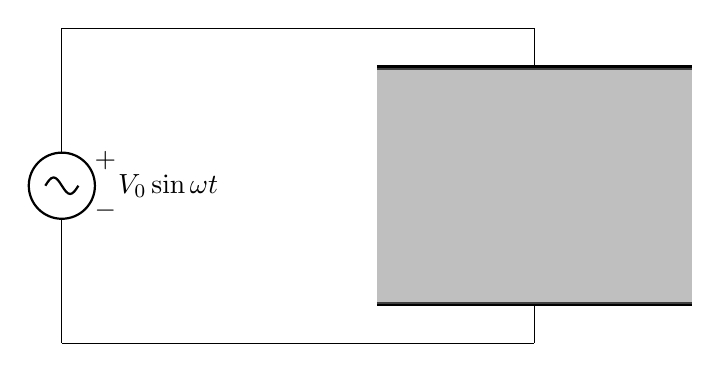
\begin{tikzpicture}
			\def\a{2};
			\def\d{3};
			\def\L{4};
			\def\F{1};
			\def\h{0.6*\d};

			\coordinate (bottom plate centre) at (3*\a,-\d/2);
			\coordinate (top plate centre) at (3*\a,\d/2);

			\begin{scope}[ultra thick]
				\draw ($ (bottom plate centre) + (-\a,0) $) -- ($ (bottom plate centre) + (\a,0) $);
				\draw ($ (top plate centre) + (-\a,0) $) -- ($ (top plate centre) + (\a,0) $);
			\end{scope}

			\begin{scope}
				\draw (bottom plate centre) -- (3*\a,-\L/2);
				\draw (top plate centre) -- (3*\a,\L/2);

				\draw (0,-\L/2) -- (3*\a,-\L/2);
				\draw (0,\L/2) -- (3*\a,\L/2);

				\draw (0,\L/2) to [sV= $V_0 \sin \omega t$] (0,-\L/2);
			\end{scope}
			\begin{scope}
				\fill [gray, opacity = 0.5] ($ (bottom plate centre) + (-\a,0) $) rectangle ($ (top plate centre) + (\a,0) $);
			\end{scope}
		\end{tikzpicture}
	\end{figure}
\end{question}

\begin{solution}
	Let the electric field inside the capacitor be $E$.
	Let $E$ be directed upwards, i.e. in the $\hat{z}$ direction.\\
	\begin{align*}
		\overrightarrow{E}            & = \frac{V}{d} \hat{z}                 \\
                                              & = \frac{V_0 \sin \omega t}{d} \hat{z} \\
		\therefore \overrightarrow{j} & = \sigma \overrightarrow{E}           \\
                                              & = \frac{\sigma V_0 \sin \omega t}{d} \hat{z}
	\end{align*}
	Consider a virtual Ampereian loop with radius $r$ inside the capacitor.\\
	Therefore, by \nameref{Maxwell's_Correction_to_Ampere's_Law},
	\begin{align*}
		\oint\limits_{\partial S} \overrightarrow{B} \cdot \overrightarrow{\dif l} & = \mu_0 \iint\limits_{S} \overrightarrow{j} \cdot \dif \overrightarrow{A} + \mu_0 \varepsilon_0 \dod{}{t}\iint\limits_{S} \overrightarrow{E} \cdot \dif \overrightarrow{A} \\
                                                                                           & = \mu_0 \frac{\sigma V_0 \sin \omega t}{d} \pi r^2 + \mu_0 \varepsilon_0 \dod{}{t}\left( \frac{V_0 \sin \omega t}{d} \pi r^2 \right)                                       \\
		\therefore 2 \pi r B                                                       & = \frac{V_0 \mu_0 \pi r^2}{d} \left( \sigma \sin \omega t + \varepsilon_0 \omega \cos \omega t \right)                                                                     \\
		\therefore B                                                               & = \frac{V_0 \mu_0 r}{2 d} (\sigma \sin \omega t + \varepsilon_0 \omega \cos \omega t)
	\end{align*}
\end{solution}

\section{Magnetism in Materials}

\begin{definition}[Paramagnetic material]
	A material which is repelled by an external magnetic field is called a paramagnetic material.
\end{definition}

\begin{definition}[Diamagnetic material]
	A material which is repelled by an external magnetic field is called a diamagnetic material.
\end{definition}

\begin{definition}[Ferromagnetic material]
	A material which is magnetized by an external magnetic field and remains magnetized after the external field is removed is called a ferromagnetic material.
\end{definition}

\newpage
\part{Electromagnetic Waves}

\section{Wave Impulse}

Let $\psi(x,t)$ be a equation representing a wave.\\
Let the speed of propagation of the wave be $\pm v$, depending on the direction.\\
Therefore, if the peak of the wave is at a point $x$ at time $0$, then the peak of the wave will be at a point $v t$ away from $x$, depending on the direction of the propagation of the wave.\\
\begin{figure}[H]
	\begin{tikzpicture}
		\def\xMIN{-1};
		\def\xMAX{8};
		\def\yMIN{-1};
		\def\yMAX{3};

		\def\v{2};
		\def\t{2};

		\begin{scope}[stealth-stealth, lightgray]
			\draw (\xMIN,0) -- (\xMAX,0) node [right];
			\draw (0,\yMIN) -- (0,\yMAX) node [above] {$y$};
		\end{scope}

		\begin{scope}[smooth]
			\draw (0,0) to [out = 20, in = 190] (1,2) to [out = -10, in = 160] (2,0);

			\node [above] at (1,2) {$t = 0$};
		\end{scope}

		\begin{scope}[smooth, red]
			\draw (0,0) to ({\v*\t},0) to [out = 20, in = 190] ++(1,2) to [out = -10, in = 160] ++(1,-2);
			\node [above] at ($ ({\v*\t},0) + (1,2) $) {$t$};
		\end{scope}

		\begin{scope}[|<->|, blue]
			\draw ($ (0,0) + (1,1) $) -- ($ (\v*\t,0) + (1,1) $) node [midway, fill = white] {$v t$};
		\end{scope}
	\end{tikzpicture}
\end{figure}
Let $f(x) = \psi(x,0)$.\\
Therefore,
\begin{align*}
	\psi(x,t) &= f(x \mp v t)
\end{align*}
Let
\begin{align*}
	\xi = x \mp v t
\end{align*}
Therefore, differentiating $\psi$ with respect to $x$,
\begin{align*}
	\dpd{\psi}{x} &= \dpd{f}{\xi} \dpd{\xi}{x}\\
	&= \dpd{f}{\xi}\\
	\therefore \dpd[2]{\psi}{x} &= \dpd{}{x}\left( \dpd{f}{\xi} \right)\\
	&= \dpd[2]{f}{\xi} \dpd{\xi}{x}\\
	&= \dpd[2]{f}{\xi}
\end{align*}
Differentiating $\psi$ with respect to $t$,
\begin{align*}
	\dpd{\psi}{t} &= \dpd{f}{\xi} \dpd{\xi}{t}\\
	&= \dpd{f}{\xi} (\mp v)\\
	\therefore \dpd[2]{\psi}{t} &= \dpd{}{t}\left( \dpd{f}{\xi} (\mp v) \right)\\
	&= (\mp v) \dpd{}{t} \left( \dpd{f}{\xi} \right)\\
	&= (\mp v) \dpd[2]{f}{\xi} \dpd{\xi}{t}\\
	&= (\mp v) \dpd[2]{f}{\xi} (\mp v)\\
	&= v^2 \dpd[2]{f}{\xi}
\end{align*}
Therefore,
\begin{align*}
	\dpd[2]{\psi}{x} &= \frac{1}{v^2} \dpd[2]{\psi}{t}
\end{align*}

\section{1D Waves}

Let
\begin{align*}
	\psi(x,t) &= A \cos\left( k (x - v t) + \varphi_0 \right)\\
	&= A \cos\left( k x - \omega t + \varphi_0 \right)
\end{align*}
$A$ is called the amplitude.\\
$k$ is called the wave number.\\
$v$ is the propagation speed.
It is dependent on the medium of propagation only.\\
$\omega = k v$ is called the angular frequency.\\
$T = \frac{2 \pi}{\omega}$ is called the time period.\\
$f = \nu = \frac{1}{T} = \frac{\omega}{2 \pi}$ is called the time frequency.\\
$\varphi_0$ is called the initial phase.\\
$\lambda = \frac{2 \pi}{k}$ is called the wavelength of the wave.

\section{3D Waves}

Let $\hat{n}$ be the unit vector in the direction of the propagation of the wave.\\
Therefore, the equation of the wave
\begin{align*}
	\psi\left( \overrightarrow{r} , t \right) &= f\left( \hat{n} \cdot \overrightarrow{r} - v t \right)\\
	&= A \cos\left( k \left( \hat{n} \cdot \overrightarrow{r} - v t \right) + \varphi_0 \right)\\
	&= A \cos\left( \overrightarrow{k} \cdot \overrightarrow{r} - \omega t + \varphi_0 \right)
\end{align*}
$\overrightarrow{k} = k \hat{n}$ is called the wave vector.\\
Therefore,
\begin{align*}
	\nabla^2 \psi &= \frac{1}{v^2} \dpd[2]{\psi}{t}
\end{align*}

\section{Electromagnetic Waves}

For $\overrightarrow{E}$ and $\overrightarrow{B}$, in vacuum, Maxwell's Equations are
\begin{align*}
	\overrightarrow{\nabla} \cdot \overrightarrow{E} &= 0\\
	\overrightarrow{\nabla} \times \overrightarrow{E} &= -\dpd{B}{t}\\
	\overrightarrow{\nabla} \cdot \overrightarrow{B} &= 0\\
	\overrightarrow{\nabla} \times \overrightarrow{E} &= \mu_0 \varepsilon_0 \dpd{E}{t}
\end{align*}
Therefore,
\begin{align*}
	\overrightarrow{\nabla} \times \overrightarrow{E}                                    & = \mu_0 \varepsilon_0 \dpd{E}{t}                                                                                        \\
	\therefore \dpd{}{t}\left( \overrightarrow{\nabla} \times \overrightarrow{B} \right) & = \dpd{}{t}\left( \mu_0 \varepsilon_0 \dpd{\overrightarrow{E}}{t} \right)                                               \\
	\therefore \overrightarrow{\nabla} \times \dpd{\overrightarrow{B}}{t}                & = \mu_0 \varepsilon_0 \dpd[2]{\overrightarrow{E}}{t}                                                                    \\
	\therefore \mu_0 \varepsilon_0 \dpd[2]{\overrightarrow{E}}{t}                        & =  \overrightarrow{\nabla} \times \left( \overrightarrow{\nabla} \times \overrightarrow{E} \right)                      \\
                                                                                             & = -\overrightarrow{\nabla} \times \left( \overrightarrow{\nabla} \times \overrightarrow{E} \right)                      \\
                                                                                             & = -\overrightarrow{\nabla} \cancelto{0}{\left( \overrightarrow{\nabla} \cdot \overrightarrow{E} \right)} + \nabla^2 \overrightarrow{E} \\
                                                                                             & = \nabla^2 \overrightarrow{E}                                                                                           \\
\end{align*}
Similarly for $\overrightarrow{B}$.\\
Therefore,
\begin{align*}
	\nabla^2 \overrightarrow{E} &= \mu_0 \varepsilon_0 \dpd[2]{\overrightarrow{E}}{t}\\
	\nabla^2 \overrightarrow{B} &= \mu_0 \varepsilon_0 \dpd[2]{\overrightarrow{B}}{t}
\end{align*}
Therefore, both $\overrightarrow{E}$ and $\overrightarrow{B}$ satisfy 3D wave equations.\\
Hence the electric an magnetic fields are waves.

\subsection{Direction of EM Wave Propagation}

\begin{align*}
	\overrightarrow{E} &= \overrightarrow{E_0} f\left( \hat{n} \cdot \overrightarrow{r} - c t \right)\\
	&= \overrightarrow{E_0} f(n_x x + n_y y + n_z z - c t)\\
	\overrightarrow{B} &= \overrightarrow{B_0} f\left( \hat{n} \cdot \overrightarrow{r} - c t \right)\\
	&= \overrightarrow{B_0} f(n_x x + n_y y + n_z z - c t)\\
\end{align*}
By Maxwell's Equations,
\begin{align*}
	0 &=\overrightarrow{\nabla} \cdot \overrightarrow{E}\\
	&= \overrightarrow{\nabla} \left( \overrightarrow{E_0} f(n_x x + n_y y + n_z z - c t) \right)\\
	&= \cancelto{0}{\left( \overrightarrow{\nabla} \cdot \overrightarrow{E_0} \right)} f(n_x x + n_y y + n_z z - c t) + \overrightarrow{E_0} \cdot \overrightarrow{\nabla} f(n_x x + n_y y + n_z z - c t)\\
	&= \overrightarrow{E_0} \cdot \hat{n} f'
\end{align*}
Therefore, as the cross product is zero, $\overrightarrow{E_0} \perp \hat{n}$.\\
Similarly, as $\overrightarrow{\nabla} \cdot \overrightarrow{B} = 0$, $\overrightarrow{B_0} \perp \hat{n}$.

\subsection{Mutual Perpendicularity of $\overrightarrow{E}$ and $\overrightarrow{B}$}

\begin{align*}
	-\dpd{\overrightarrow{B}}{t} &= \overrightarrow{\nabla} \times \overrightarrow{E}\\
	&= \overrightarrow{\nabla} \times \left( \overrightarrow{E_0} \cdot f \right)\\
	&= \cancelto{0}{\left( \overrightarrow{\nabla} \times \overrightarrow{E_0} \right)} f - \overrightarrow{E_0} \times \overrightarrow{\nabla} f\\
	&= -\overrightarrow{E_0} \times f' \hat{n}\\
	\therefore -\overrightarrow{B_0} \cdot f' \cdot (-c) &= -\overrightarrow{B_0} \times f' \hat{n}\\
	\therefore \hat{n} \times \overrightarrow{E_0} &= \overrightarrow{B_0} c
\end{align*}
Therefore, $\overrightarrow{E}$ and $\overrightarrow{B}$ are mutually perpendicular, and $E_0 = c B_0$.

\subsection{Electromagnetic Energy Density}

The electromagnetic energy density in vacuum is
\begin{align*}
	u_{\textnormal{em}} &= \frac{1}{2} \varepsilon_0 E^2 + \frac{1}{2} \frac{1}{\mu_0} B^2\\
	&= \frac{1}{2} \varepsilon_0 E^2 + \frac{1}{2 \mu_0} \left( \frac{E}{c} \right)^2\\
	\intertext{As $c^2 = \frac{1}{\mu_0 \varepsilon_0}$,}
	u_{\textnormal{em}} &= \frac{1}{2} \varepsilon_0 E^2 + \frac{1}{2 \mu_0} \frac{E^2}{\frac{1}{\mu_0 \varepsilon_0}}\\
	&= \frac{1}{2} \varepsilon_0 E^2 + \frac{1}{2} \varepsilon_0 E^2\\
	&= \varepsilon_0 E^2\\
	&= c \varepsilon_0 E B
\end{align*}

\subsection{Poynting Vector}

\begin{definition}[Poynting vector]
	\begin{align*}
		\overrightarrow{s} &= u_{\textnormal{em}} C \hat{n}\\
		&= c^2 \varepsilon_0 E B \hat{n} \\
		&= \frac{E B}{\mu_0} \hat{n}\\
		&= \frac{\overrightarrow{E} \times \overrightarrow{B}}{\mu_0}
	\end{align*}
	is called the Poynting vector.
\end{definition}

\begin{question}
	A cylindrical resistor of resistance $R$ has length $L$ and radius $a$.\\
	The resistor is kept on the $z$ axis.\\
	A current $I$ is flowing in the $\hat{z}$ direction.\\
	The voltage across the resistor is $V$.\\
	Show that the total flux of $\overrightarrow{S}$ through the surface of the resistor is equal to the power in the resistor.
\end{question}

\begin{solution}
	Due to the potential difference across the resistor, there is an electric field inside the resistor.
	\begin{align*}
		\overrightarrow{E} &= \frac{V}{L} \hat{z}
	\end{align*}
	Due to the current flowing through the resistor, there is a magnetic field everywhere.\\
	The magnetic field at the surface of the resistor is
	\begin{align*}
		\overrightarrow{B} &= \frac{\mu_0 I}{2 \pi a} \hat{\varphi}
	\end{align*}
	Therefore, at the surface of the resistor, the Poynting vector is
	\begin{align*}
		\overrightarrow{S} &= \frac{\overrightarrow{E} \times \overrightarrow{B}}{\mu_0}\\
		&= -\hat{r} \frac{\frac{V}{L} \frac{\mu_0 I}{2 \pi a}}{\mu_0}\\
		&= -\frac{I^2 R}{2 \pi a L} \hat{r}
	\end{align*}
	Therefore, the total flux of $\overrightarrow{S}$ through the resistor's surface is
	\begin{align*}
		\frac{I^2 R}{2 \pi a L} \cdot 2 \pi a L &= I^2 R\\
		&= P
	\end{align*}
\end{solution}

\section{Momentum due to Electromagnetic Waves}

Consider two particles of mass $m$ and charge $q$ each, moving as shown.
\begin{figure}[H]
	\begin{tikzpicture}
		\def\a{3};
		\def\F{1};

		\begin{scope}[red]
			\filldraw (0,\a) circle (2pt);
			\draw[-stealth] (0,\a) -- ++(-90:\F) node [below] {$v$};
			\draw[-stealth] (\a,0) -- ++(90:\F) node [above] {$F$};
		\end{scope}

		\begin{scope}[blue]
			\filldraw (\a,0) circle (2pt);
			\draw[-stealth] (\a,0) -- ++(180:\F) node [left] {$v$};
			\draw[-stealth] (0,\a) -- ++(0:\F) node [right] {$F$};
		\end{scope}
	\end{tikzpicture}
\end{figure}
Therefore, the magnetic force exerted by each particle on the other is as shown.\\
Therefore, the net force on the system does not cancel out.\\
Hence, Newton's Third Law is violated.\\
As a result, the Principle of Conservation of Momentum is also violated.\\
To correct this error, the momentum due to the generated electromagnetic waves is defined to be
\begin{align*}
	\overrightarrow{p_{\textnormal{em}}} &= \frac{\overrightarrow{S}}{C^2}\\
	&= \frac{u_{\textnormal{em}}}{c} \hat{n}
\end{align*}

\end{document}
